%% March 2018
%%%%%%%%%%%%%%%%%%%%%%%%%%%%%%%%%%%%%%%%%%%%%%%%%%%%%%%%%%%%%%%%%%%%%%%%%%%%
% AGUJournalTemplate.tex: this template file is for articles formatted with LaTeX
%
% This file includes commands and instructions
% given in the order necessary to produce a final output that will
% satisfy AGU requirements, including customized APA reference formatting.
%
% You may copy this file and give it your
% article name, and enter your text.
%
%
% Step 1: Set the \documentclass
%
% There are two options for article format:
%
% PLEASE USE THE DRAFT OPTION TO SUBMIT YOUR PAPERS.
% The draft option produces double spaced output.
%

%% To submit your paper:
\documentclass[draft,linenumbers]{agujournal2018}
\usepackage{apacite}
\usepackage{url} %this package should fix any errors with URLs in refs.
%%%%%%%
% As of 2018 we recommend use of the TrackChanges package to mark revisions.
% The trackchanges package adds five new LaTeX commands:
%
%  \note[editor]{The note}
%  \annote[editor]{Text to annotate}{The note}
%  \add[editor]{Text to add}
%  \remove[editor]{Text to remove}
%  \change[editor]{Text to remove}{Text to add}
%
% complete documentation is here: http://trackchanges.sourceforge.net/
%%%%%%%


%% Enter journal name below.
%% Choose from this list of Journals:
%
% JGR: Atmospheres
% JGR: Biogeosciences
% JGR: Earth Surface
% JGR: Oceans
% JGR: Planets
% JGR: Solid Earth
% JGR: Space Physics
% Global Biogeochemical Cycles
% Geophysical Research Letters
% Paleoceanography and Paleoclimatology
% Radio Science
% Reviews of Geophysics
% Tectonics
% Space Weather
% Water Resources Research
% Geochemistry, Geophysics, Geosystems
% Journal of Advances in Modeling Earth Systems (JAMES)
% Earth's Future
% Earth and Space Science
% Geohealth
%
% ie, \journalname{Water Resources Research}

\journalname{Geochemistry, Geophysics, Geosystems}


% tightlist command for lists without linebreak
\providecommand{\tightlist}{%
  \setlength{\itemsep}{0pt}\setlength{\parskip}{0pt}}

% From pandoc table feature
\usepackage{longtable,booktabs,array}
\usepackage{calc} % for calculating minipage widths
% Correct order of tables after \paragraph or \subparagraph
\usepackage{etoolbox}
\makeatletter
\patchcmd\longtable{\par}{\if@noskipsec\mbox{}\fi\par}{}{}
\makeatother
% Allow footnotes in longtable head/foot
\IfFileExists{footnotehyper.sty}{\usepackage{footnotehyper}}{\usepackage{footnote}}
\makesavenoteenv{longtable}


\usepackage{pdflscape}
\newcommand{\blandscape}{\begin{landscape}}
\newcommand{\elandscape}{\end{landscape}}
\usepackage{longtable}
\usepackage{tabularx}
\usepackage{booktabs}
\usepackage{setspace}
\usepackage{caption}
\captionsetup[figure]{font={stretch=0.6}}
\usepackage{float}
\raggedbottom
\usepackage{soul}
\usepackage[utf8]{inputenc}
\usepackage{amsmath}
\usepackage{amsfonts}
\usepackage{amssymb}
\DeclareUnicodeCharacter{2212}{-}
\DeclareUnicodeCharacter{02DA}{$^\circ$}
\DeclareUnicodeCharacter{2265}{$\geq$}
\DeclareUnicodeCharacter{2264}{$\leq$}
\DeclareUnicodeCharacter{177}{$\pm$}
\providecommand{\tightlist}{\setlength{\itemsep}{0pt}\setlength{\parskip}{0pt}}
\def\tightlist{}
\usepackage{hyperref}

\begin{document}


%% ------------------------------------------------------------------------ %%
%  Title
%
% (A title should be specific, informative, and brief. Use
% abbreviations only if they are defined in the abstract. Titles that
% start with general keywords then specific terms are optimized in
% searches)
%
%% ------------------------------------------------------------------------ %%

% Example: \title{This is a test title}

\title{RocMLMs: Predicting Rock Properties through Machine Learning Models}

%% ------------------------------------------------------------------------ %%
%
%  AUTHORS AND AFFILIATIONS
%
%% ------------------------------------------------------------------------ %%

% Authors are individuals who have significantly contributed to the
% research and preparation of the article. Group authors are allowed, if
% each author in the group is separately identified in an appendix.)

% List authors by first name or initial followed by last name and
% separated by commas. Use \affil{} to number affiliations, and
% \thanks{} for author notes.
% Additional author notes should be indicated with \thanks{} (for
% example, for current addresses).

% Example: \authors{A. B. Author\affil{1}\thanks{Current address, Antartica}, B. C. Author\affil{2,3}, and D. E.
% Author\affil{3,4}\thanks{Also funded by Monsanto.}}

\authors{
Buchanan Kerswell
\affil{1}
Nestor Cerpa
\affil{1}
Andréa Tommasi
\affil{1}
Marguerite Godard
\affil{1}
José Alberto Padrón-Navarta
\affil{2}
}


% \affiliation{1}{First Affiliation}
% \affiliation{2}{Second Affiliation}
% \affiliation{3}{Third Affiliation}
% \affiliation{4}{Fourth Affiliation}

\affiliation{1}{Géosciences Montpellier, Université de Montpellier \& CNRS, Montpellier, France}
\affiliation{2}{Instituto Andaluz de Ciencias de la Tierra, CSIC--UGR, Granada, Spain}
%(repeat as many times as is necessary)

%% Corresponding Author:
% Corresponding author mailing address and e-mail address:

% (include name and email addresses of the corresponding author.  More
% than one corresponding author is allowed in this LaTeX file and for
% publication; but only one corresponding author is allowed in our
% editorial system.)

% Example: \correspondingauthor{First and Last Name}{email@address.edu}
\correspondingauthor{Buchanan Kerswell}{\href{mailto:buchanan.kerswell@umontpellier.fr}{\nolinkurl{buchanan.kerswell@umontpellier.fr}}}

%% Keypoints, final entry on title page.

%  List up to three key points (at least one is required)
%  Key Points summarize the main points and conclusions of the article
%  Each must be 100 characters or less with no special characters or punctuation

% Example:
% \begin{keypoints}
% \item	List up to three key points (at least one is required)
% \item	Key Points summarize the main points and conclusions of the article
% \item	Each must be 100 characters or less with no special characters or punctuation
% \end{keypoints}

\begin{keypoints}
\item RocMLMs predict rock properties up to 10\(^1\)--10\(^3\) faster than commonly used methods
\item RocMLMs trained with Neural Networks are more efficient compared to other regression algorithms
\item RocMLM training data show good agreement with PREM and STW105 for an average mantle geotherm
\end{keypoints}

%% ------------------------------------------------------------------------ %%
%
%  ABSTRACT
%
% A good abstract will begin with a short description of the problem
% being addressed, briefly describe the new data or analyses, then
% briefly states the main conclusion(s) and how they are supported and
% uncertainties.
%% ------------------------------------------------------------------------ %%

%% \begin{abstract} starts the second page

\begin{abstract}
Mineral phase transformations significantly alter the bulk density and elastic properties of mantle rocks and consequently have profound effects on mantle dynamics and seismic wave propagation. These changes in the physical properties of mantle rocks result from evolution in the equilibrium mineralogical composition, which can be predicted by the minimization of the Gibbs Free Energy with respect to pressure (P), temperature (T), and chemical composition (X). Thus, numerical models that simulate mantle convection and/or probe the elastic structure of the Earth's mantle must account for varying mineralogical compositions to be self-consistent. Yet coupling Gibbs Free Energy minimization (GFEM) approaches with numerical geodynamic models is currently intractable for high-resolution simulations because execution speeds of widely-used GFEM programs (10\(^0\)--10\(^2\) ms) are impractical in many cases. As an alternative, this study introduces machine learning models (RocMLMs) that have been trained to predict thermodynamically self-consistent rock properties at arbitrary PTX conditions between 1--28 GPa, 773--2273 K, and mantle compositions ranging from fertile (lherzolitic) to refractory (harzburgitic) end-members defined with a large dataset of published mantle compositions. RocMLMs are 10\(^1\)--10\(^3\) times faster than GFEM calculations or GFEM-based look-up table approaches with equivalent accuracy. Depth profiles of RocMLMs predictions are nearly indistinguishable from reference models PREM and STW105, demonstrating good agreement between thermodynamic-based predictions of density, Vp, and Vs and geophysical observations. RocMLMs are therefore capable, for the first time, of emulating dynamic evolution of density, Vp, and Vs in high-resolution numerical geodynamic models.
\end{abstract}
\noindent{\bf Plain language summary}\vskip-\parskip

\noindent{The mineralogical makeup of rocks within Earth's mantle largely determines how the mantle flows over geologic time, and how it responds to seismic waves triggered by earthquakes, because mineral assemblages control important rock properties such as density and stiffness (elasticity). The mineralogy of mantle rocks is not constant, however. It changes depending on three factors: pressure, temperature, and the chemical composition of the rock. Thus, it is important for computer simulations of mantle convection to account for the evolution of rock mineralogy in time and space. Computer programs that can predict rock properties based on thermodynamic calculations of the most stable mineral assemblages are available, but these programs are generally too slow to be used in an iterative manner in high-resolution computer simulations of mantle convection. As an alternative approach, this study introduces machine learning models (RocMLMs) that have ``learned'' how to predict rock properties (density and elasticity) for a large range of mantle rock compositions and pressure-temperature conditions by ``training'' on a large dataset of thermodynamic calculations. We demonstrate that RocMLMs can then predict rock properties up to 10\(^1\)--10\(^3\) times faster than state-of-the-art methods. We tested RocMLM predictions against reference mantle models based on observations of seismic waves and found good agreement. RocMLMs are therefore capable of fast and highly-accurate predictions of changes in rock properties and can be implemented in high-resolution computer simulations of mantle convection.}
\vskip18pt
\section{Introduction}\label{introduction}

The dominant mineral phases in Earth's mantle are olivine, pyroxene, garnet, wadsleyite, ringwoodite, bridgmanite, ferropericlase, calcium silicate perovskite, and MgSiO\(_3\) post-perovskite \citep[e.g.,][]{stixrude2012}. Mantle mineralogy evolves with depth by a series of relatively discontinuous phase transformations that define sharp transitions in the physical properties of mantle rocks \citep{ringwood1991}. The most important phase transformations occur at depths between 410 km and 670 km beneath Earth's surface, defining the transition from the upper to the lower mantle (Equation \eqref{eq:mantle-transitions}). This mantle transition zone (MTZ) is characterized by sharp variations in density and elastic properties that strongly impact mantle convection \citep{christensen1995, fukao2001, jenkins2016, karato2001, kuritani2019, nakagawa2005, ringwood1991, schubert1975, tackley1994, wang2015}, and the propagation of teleseismic waves \citep{dziewonski1981, ita1992, ringwood1991}. The MTZ is therefore an essential feature for modeling mantle structure and dynamics. With respect to a simple FeO-MgO-SiO\(_2\) chemical system, the most important MTZ reactions can be written as:

\begin{align}
    \text{olivine} \xrightarrow{\text{410 km}} \text{wadsleyite} &\rightarrow \text{ringwoodite} \xrightarrow{\text{670 km}} \text{bridgmanite} + \text{ferropericlase} \notag \\
    \text{(Mg,Fe)}_{2}\text{SiO}_{4} \rightarrow \text{(Mg,Fe)}_{2}\text{SiO}_{4} &\rightarrow \text{(Mg,Fe)}_{2}\text{SiO}_{4} \rightarrow \text{(Mg,Fe)}\text{SiO}_{3} + \text{(Mg,Fe)}\text{O}
    \label{eq:mantle-transitions}
\end{align}

These phase changes (e.g., Equation \eqref{eq:mantle-transitions}) are often parameterized in numerical geodynamic simulations with simple pressure-temperature (PT)-dependent reaction boundaries based on high-pressure experiments \citep[e.g.,][]{agrusta2017, ballmer2015, christensen1995, civzkova2013, kerswell2021, liu1991, nakagawa2005, tackley1994, torii2007}. Alternatively, some numerical geodynamic experiments \citep[e.g.,][]{li2019, yang2020} use Gibbs Free Energy minimization (GFEM) programs \citep[e.g.,][]{connolly2009, riel2022} to precompute Lookup Tables of rock properties, which are subsequently referenced to adjust material properties as the numerical experiments evolve. These implementations usually consider fixed ideal mantle compositions, such as pyrolite, and/or approximate phase transitions with simple functions. These approaches neglect the PT dependency of mineral transitions on natural variations of mantle composition (X) such as variations of Fe-Mg and Al-Ca that may be either primordial or result from melt extraction or reactions during melt transport. Despite these simplifications, these models have corroborated that the MTZ is a critical feature impacting subduction dynamics, mantle plume dynamics, and water cycling in the deep Earth.

More self-consistent numerical models of mantle convection would track changes in physical properties of mantle rocks by computing GFEM as a function of the evolution of PTX conditions. However, this is currently intractable for high-resolution geodynamic models because GFEM programs remain too slow (≥ 4--228 ms per PTX point) to be applied recursively during a geodynamic simulation (see Supporting Information). Parallelization of GFEM programs can increase efficiency by scaling the number of parallel processes \citep{riel2022}, but continuously computing phase relations during geodynamic simulations would require GFEM efficiency on the order of ≤ 10\(^0\)--10\(^{-1}\) ms to be feasible (see Supporting Information), which may be difficult to achieve solely by parallelisation and/or direct improvements to the current GFEM paradigm.

Here, we propose an alternative approach to predicting rock properties based on the use of machine learning models (referred to as RocMLMs) that have been ``trained'' on a multidimensional dataset of precomputed rock properties using classical (k-Neighbors, Decision Trees) and deep (Neural Network) regression algorithms. These later regression algorithms compress large amounts of thermodynamic information into highly efficient nonlinear functions, allowing RocMLMs to infer (predict) rock properties across arbitrary PTX conditions faster than any current GFEM algorithm. We demonstrate that RocMLMs are thus highly efficient emulators of GFEM programs and are well-suited for predicting bulk rock properties in numerical geodynamic models.

This article begins by detailing our method for building, training, and evaluating RocMLMs. We then demonstrate that RocMLMs can predict densities and seismic velocities in a dry upper mantle and transition zone up to 10\(^1\)--10\(^3\) times faster than commonly used GFEM programs with equivalent accuracies. Finally, we compare RocMLM predictions with reference models derived from seismological datasets \citep{dziewonski1981, kustowski2008} and discuss the accuracy and performance of RocMLMs with respect to their future implementation in numerical geodynamic models.

\section{Methods}\label{sec:methods}

The following sections describe the methodologies employed in constructing, training, and assessing RocMLMs, with a focus on four primary objectives. First, define the size and scope of RocMLM training data to ensure widespread applicability of RocMLMs to the upper mantle and transition zone (Section \ref{sec:training-data-design}). Second, define a generalized approach for generating RocMLM training data to ensure applicability to any GFEM program (e.g., MAGEMin, Perple\_X, and others, Section \ref{sec:generate-training-data}). Third, train RocMLMs on a set of input features that can be routinely computed during geodynamic simulations to ensure widespread applicability of RocMLMs to various geodynamic codes (Section \ref{sec:train-rocmlms}). Fourth, rank the overall performance of RocMLMs in terms of accuracy and efficiency (Section \ref{sec:evaluate-rocmlms}).

\subsection{RocMLM Training Dataset Design}\label{sec:training-data-design}

\subsubsection{Pressure-Temperature Conditions}\label{sec:pt-conditions}

High-pressure experiments constrain the reaction olivine → wadsleyite between 14.0 ± 1.0 GPa and 1600 ± 400 K with Clapeyron slopes between 2.4x10\(^{−3}\) ± 1.4x10\(^{−3}\) GPa/K \citep{akaogi1989, katsura1989, li2019, morishima1994}. Likewise, the reaction ringwoodite → bridgmanite + ferropericlase is constrained between 24.0 ± 1.5 GPa and 1600 ± 400 K with negative Clapeyron slopes between -2.0x10\(^{−3}\) ± 1.6x10\(^{−3}\) GPa/K \citep{akaogi2007, bina1994, hirose2002, ishii2018, ito1982, ito1990, ito1989a, ito1989b, katsura2003, litasov2005}. We therefore compute RocMLM training data within a rectangular PT region bounded between 1--28 GPa and 773--2273 K to encompass expected conditions for the entire upper mantle and MTZ---from approximately 30 km to 865 km depth (Figure \ref{fig:training-dataset-design}).

Figure \ref{fig:training-dataset-design} shows that our training dataset PT range includes PT conditions that are not expected to exist in neither the Earth's mantle, nor geodynamic simulations \citep[e.g., very cold conditions with thermal gradients ≤ 5 K/km,][]{cerpa2022, maruyama1996, syracuse2010}. Such a large rectangular PT range might be considered impractical with respect to training efficiency (unnecessary amounts of training data) and accuracy (outside the bounds of calibrated thermodynamic data) compared to an irregular PT range bounded between arbitrary geotherms. However, initial sensitivity tests showed comparable RocMLM performance irrespective of the range of PT conditions used to generate RocMLM training data. Thus, we adopted a regular rectangular training dataset design because it is computationally convenient and does not deteriorate RocMLM accuracy.



\begin{figure}[htbp]

{\centering 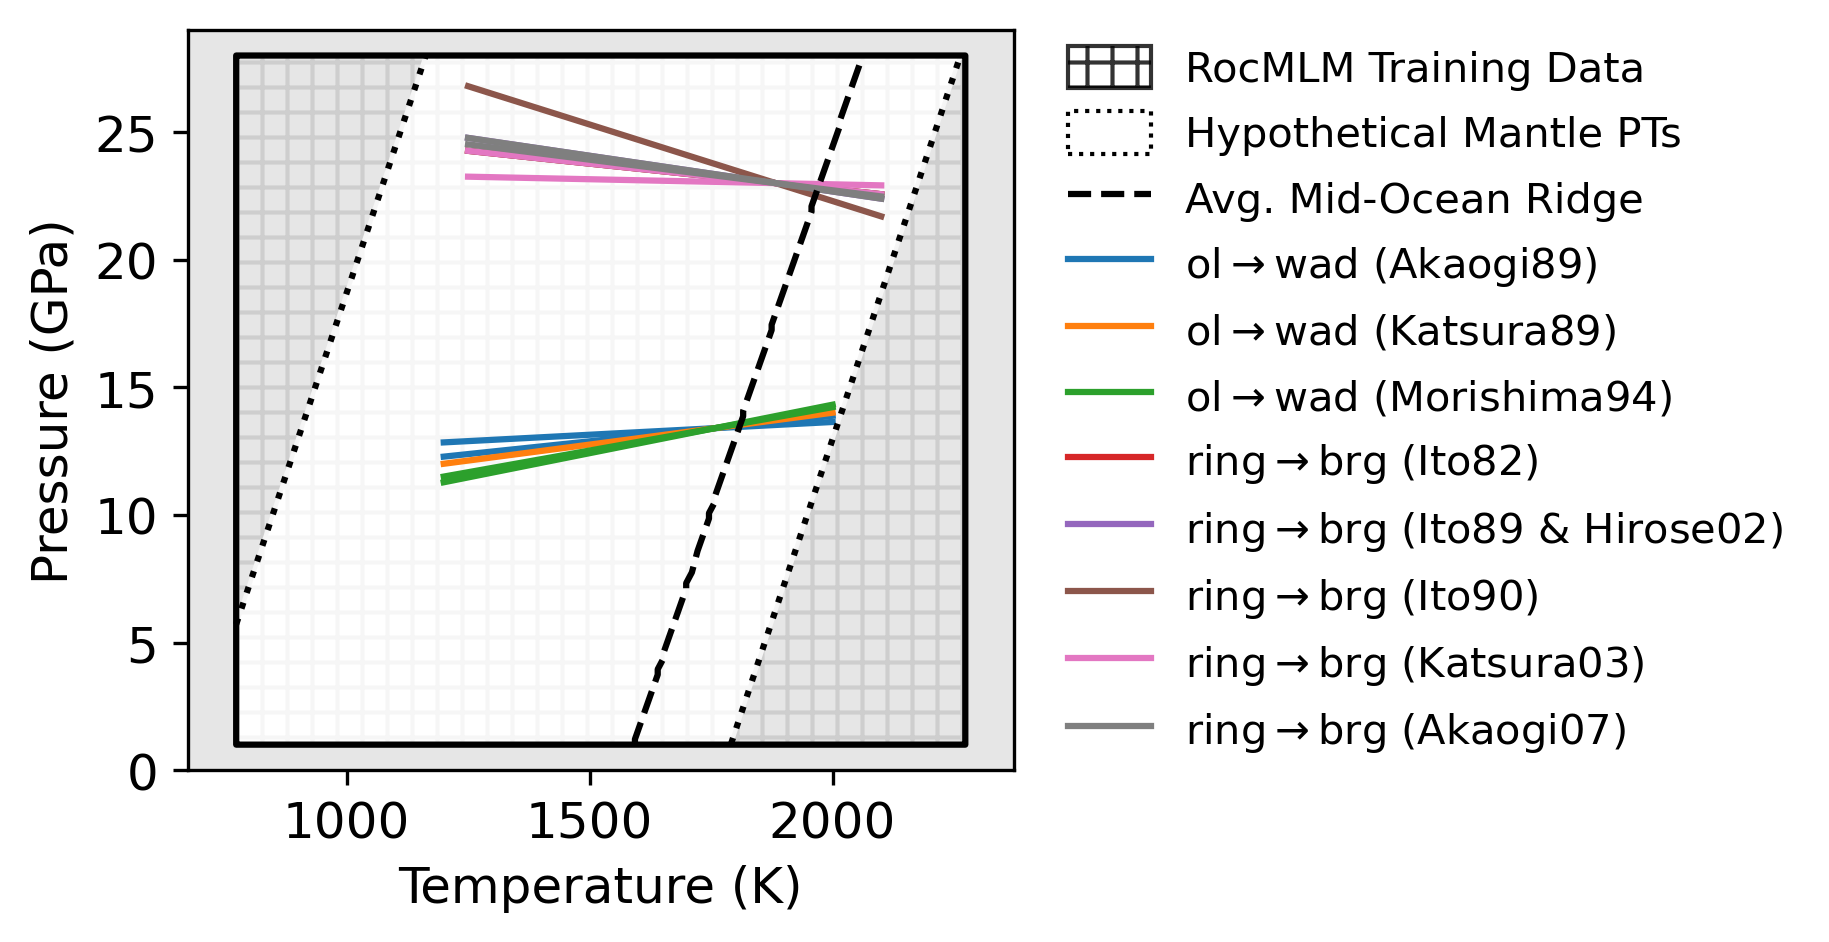
\includegraphics[width=1\linewidth,]{training-dataset-design} 

}

\caption{PT diagram showing the range of conditions considered for generating RocMLM training data (hatched region) compared to a range of possible upper mantle conditions (inner white region). The dotted black lines are geotherms with arbitrary mantle potential temperatures of 673 K and 1773 K and a constant adiabatic gradient of 0.5 K/km, representing hypothetical lower and upper bounds for mantle PT conditions (including hypothetical cold lithospheric slabs). The dashed black line is an average geotherm for a mid-ocean ridge (1573 K adiabat). Phase boundaries for the 410 km and 670 km discontinuities (colored lines) are from a compilation by \citet{li2019}.}\label{fig:training-dataset-design}
\end{figure}

\subsubsection{Bulk Mantle Compositions}\label{sec:bulk-rock-compositions}

We derived an array of synthetic bulk mantle compositions with the aim of encompassing the widest range of chemical variability in Earth's mantle. For this, we applied a statistical analysis to publicly-available geochemical data from thousands of natural peridotite samples. The procedure was as follows.

Bulk chemical analyses of peridotite samples were downloaded using the Earthchem.org Search Portal with a single search criterion: \emph{``set sample type \textgreater{} igneous rocks \textgreater{} names from Earthchem categories \textgreater{} igneous-plutonic-ultramafic''}. The search queried 19791 samples with rock type classifications that we did not modify from their original labels. Samples lacking analyses for SiO\(_2\), MgO, Al\(_2\)O\(_3\), or CaO were excluded from the dataset. All samples classified as ``unknown'', chromitite, limburgite, wehrlite, undifferentiated peridotite, dunite, or pyroxenite were also excluded from the dataset to focus on samples that are most likely mantellic, that is, residues of partial melting modified (or not) by refertilization, rather than products of fractional crystallization (Bowen, 1915). The data were grouped according to the remaining rock types (lherzolite and harzburgite) and outliers were removed from each group using a 1.5 interquartile range threshold applied to each chemical component. Cr and Ni measured as minor elements (ppm) were converted to Cr\(_2\)O\(_3\) and NiO (wt.\%) and all Fe oxides were converted to Fe\(_2\)O\(_3\)T. Total oxides were then checked against H\(_2\)O, CO\(_2\), and LOI to determine if chemical analyses were performed before or after ignition. Analyses with total oxides summing to ≤ 97\% or ≥ 103\% were considered erroneous, or otherwise low-quality, and excluded from the dataset. All analyses were then normalized to a volatile-free basis before converting Fe\(_2\)O\(_3\)T to FeOT. After normalization, the final compositional space investigated includes the components Na\(_2\)O-CaO-FeO-MgO-Al\(_2\)O\(_3\)-SiO\(_2\)-TiO\(_2\) (NCFMAST system). The final dataset contains 3111 chemical analyses of classified peridotite samples (Table \ref{tab:earthchem-counts}).

We applied Principal Component Analysis (PCA) to the standardized peridotite dataset to reduce its dimensionality from the original 7-oxides space. PCA requires complete data, so samples were first arranged by decreasing MgO and increasing SiO\(_2\) content and a k-Neighbors algorithm was applied to impute missing oxide analyses, which were mainly the Na\(_2\)O component (see Table \ref{tab:earthchem-counts} for missing analyses counts). Following common practice, a ``z-score normalization'' was applied to all oxide components before running PCA. The first two principal components (PC1 and PC2) explain 78\% of the variance of the dataset, which we considered to be sufficient for modeling a broad range of peridotitic mantle compositions. PC1 separates samples by their TiO\(_2\), Al\(_2\)O\(_3\), MgO, CaO, and Na\(_2\)O contents, while PC2 separates samples by SiO\(_2\) and FeO (Figure \ref{fig:earthchem-mixing-array}).

In this PC space, we drew a mixing line connecting the lherzolite and harzburgite group centroids (i.e., the median values for PC1 and PC2 for each group). The lherzolite-harzburgite mixing line was then extended until reaching the approximate location of the most fertile (Al\(_2\)O\(_3\)-CaO-TiO\(_2\)-rich) and most refractory (MgO-rich, SiO\(_2\)-poor) peridotite samples, hereafter referred to as Primitive Synthetic Upper Mantle (PSUM) and Depleted Synthetic Upper Mantle (DSUM, Figure \ref{fig:earthchem-mixing-array}b), respectively. The mixing line approximates the widest array of mantle compositions derived from the natural rock record and may be interpreted as representing the first order composition variation in response to melt extraction (depletion) or addition (refertilization) in the mantle. The mixing line therefore provides a basis for sampling synthetic bulk mantle compositions directly from PC space, which were then used to generate RocMLM training data.

\begin{longtable}[]{@{}
  >{\raggedright\arraybackslash}p{(\columnwidth - 16\tabcolsep) * \real{0.1102}}
  >{\raggedleft\arraybackslash}p{(\columnwidth - 16\tabcolsep) * \real{0.1017}}
  >{\raggedleft\arraybackslash}p{(\columnwidth - 16\tabcolsep) * \real{0.0932}}
  >{\raggedleft\arraybackslash}p{(\columnwidth - 16\tabcolsep) * \real{0.1102}}
  >{\raggedleft\arraybackslash}p{(\columnwidth - 16\tabcolsep) * \real{0.1102}}
  >{\raggedleft\arraybackslash}p{(\columnwidth - 16\tabcolsep) * \real{0.1186}}
  >{\raggedleft\arraybackslash}p{(\columnwidth - 16\tabcolsep) * \real{0.1356}}
  >{\raggedleft\arraybackslash}p{(\columnwidth - 16\tabcolsep) * \real{0.1102}}
  >{\raggedleft\arraybackslash}p{(\columnwidth - 16\tabcolsep) * \real{0.1102}}@{}}
\caption{\label{tab:earthchem-counts} Summary of the filtered and standardized peridotite dataset from Earthchem.org. Columns with an asterisk are in wt.\%. Std = standard deviation, IQR = interquartile range.}\tabularnewline
\toprule\noalign{}
\begin{minipage}[b]{\linewidth}\raggedright
Oxide
\end{minipage} & \begin{minipage}[b]{\linewidth}\raggedleft
Measured
\end{minipage} & \begin{minipage}[b]{\linewidth}\raggedleft
Missing
\end{minipage} & \begin{minipage}[b]{\linewidth}\raggedleft
Min\(^{*}\)
\end{minipage} & \begin{minipage}[b]{\linewidth}\raggedleft
Max\(^{*}\)
\end{minipage} & \begin{minipage}[b]{\linewidth}\raggedleft
Mean\(^{*}\)
\end{minipage} & \begin{minipage}[b]{\linewidth}\raggedleft
Median\(^{*}\)
\end{minipage} & \begin{minipage}[b]{\linewidth}\raggedleft
Std\(^{*}\)
\end{minipage} & \begin{minipage}[b]{\linewidth}\raggedleft
IQR\(^{*}\)
\end{minipage} \\
\midrule\noalign{}
\endfirsthead
\toprule\noalign{}
\begin{minipage}[b]{\linewidth}\raggedright
Oxide
\end{minipage} & \begin{minipage}[b]{\linewidth}\raggedleft
Measured
\end{minipage} & \begin{minipage}[b]{\linewidth}\raggedleft
Missing
\end{minipage} & \begin{minipage}[b]{\linewidth}\raggedleft
Min\(^{*}\)
\end{minipage} & \begin{minipage}[b]{\linewidth}\raggedleft
Max\(^{*}\)
\end{minipage} & \begin{minipage}[b]{\linewidth}\raggedleft
Mean\(^{*}\)
\end{minipage} & \begin{minipage}[b]{\linewidth}\raggedleft
Median\(^{*}\)
\end{minipage} & \begin{minipage}[b]{\linewidth}\raggedleft
Std\(^{*}\)
\end{minipage} & \begin{minipage}[b]{\linewidth}\raggedleft
IQR\(^{*}\)
\end{minipage} \\
\midrule\noalign{}
\endhead
\bottomrule\noalign{}
\endlastfoot
SiO\(_2\) & 3111 & 0 & 36.7 & 52 & 44.1 & 44.1 & 1.16 & 1.24 \\
TiO\(_2\) & 2835 & 276 & 0 & 0.268 & 0.051 & 0.03 & 0.05 & 0.068 \\
Al\(_2\)O\(_3\) & 3111 & 0 & 0.023 & 4.95 & 1.65 & 1.31 & 1.14 & 1.82 \\
FeOT & 3111 & 0 & 5.98 & 15.3 & 8.05 & 8.01 & 0.675 & 0.569 \\
MgO & 3111 & 0 & 31.8 & 50.8 & 43 & 43.6 & 2.96 & 4.38 \\
CaO & 3111 & 0 & 0.01 & 5.2 & 1.46 & 1.17 & 1.04 & 1.66 \\
Na\(_2\)O & 2008 & 1103 & 0 & 0.525 & 0.127 & 0.098 & 0.11 & 0.171 \\
\end{longtable}

\subsubsection{Reducing Bulk Mantle Compositions to a Single Fertility Index Value}\label{sec:melt-fractions}

Training RocMLMs with either 7 oxide components or two PCs as inputs is possible. However, our targeted application (e.g., implementing RocMLMs in geodynamic codes) discourages the use of the two options because in either case it would require tracking the oxides in numerical geodynamic codes, which is currently impractical. Thus, we aimed to reduce the dimensionality of the training dataset from nine dimensions (7 oxide components + PT) to three dimensions (1 compositional dimension + PT) by estimating the amount of melt extraction (depletion) that might have produced the synthetic bulk mantle compositions in the training dataset. Assuming that all synthetic samples were derived from a PSUM source, we adopt a simple modal fractional melting model \citep[after][]{shaw1970}:

\begin{equation}
    \frac{C_{\text{TiO}_2}^s}{C_{\text{TiO}_2}^0} = R = (1 - F)^{\frac{1}{D_0} - 1}
    \label{eq:shaw-melting}
\end{equation}

\noindent where \(R\) is the ratio of the TiO\(_2\) concentration of the sample to the initial PSUM source (Table \ref{tab:benchmark-samples}), \(F\) is the melt fraction, and \(D_0\) = 0.05 is the bulk distribution coefficient for TiO\(_2\) in peridotite \citep[after][]{brown2016}. Note that unlike the dataset of natural peridotite samples, synthetic samples were drawn directly from PC space and their TiO\(_2\) concentrations (and other oxide components) change monotonically with PC1 from the initial PSUM source (Figure \ref{fig:earthchem-mixing-array}b,c). Synthetic samples therefore represent a smooth and idealized variability from fertile (PSUM) to depleted (DSUM) mantle compositions that captures the average variation in natural peridotite samples.

A Fertility Index (\(\xi\)) is calculated by rearranging Equation \eqref{eq:shaw-melting} for F and subtracting F from 1:

\begin{equation}
    \xi = 1 - F = R^{\frac{1}{(\frac{1}{D_0}) - 1}}
    \label{eq:melt-fraction}
\end{equation}

Training RocMLMs on \(\xi\) instead of seven oxide components is beneficial for two reasons: 1) it greatly increases RocMLM efficiency and 2) unlike oxide components or PCs, melt fraction is routinely implemented in numerical geodynamic simulations \citep[e.g.,][]{cerpa2019, gerya2003, kelley2010, li2019, sizova2010, yang2020}. Likewise, tracking the depletion/fertility of the mantle in geodynamics models with Lagrangian tracers and/or compositional fields is more conceivable \citep{tackley2003, cagnioncle2007, gerya2011, agrusta2015}. Although we chose \(\xi\) for RocMLM training, \(\xi\) and \(F\) represent opposite reference frames for the same time-integrated melting process, and are therefore interchangeable. This approach offers a generalized solution for coupling RocMLMs to geodynamic codes.



\begin{figure}[htbp]

{\centering 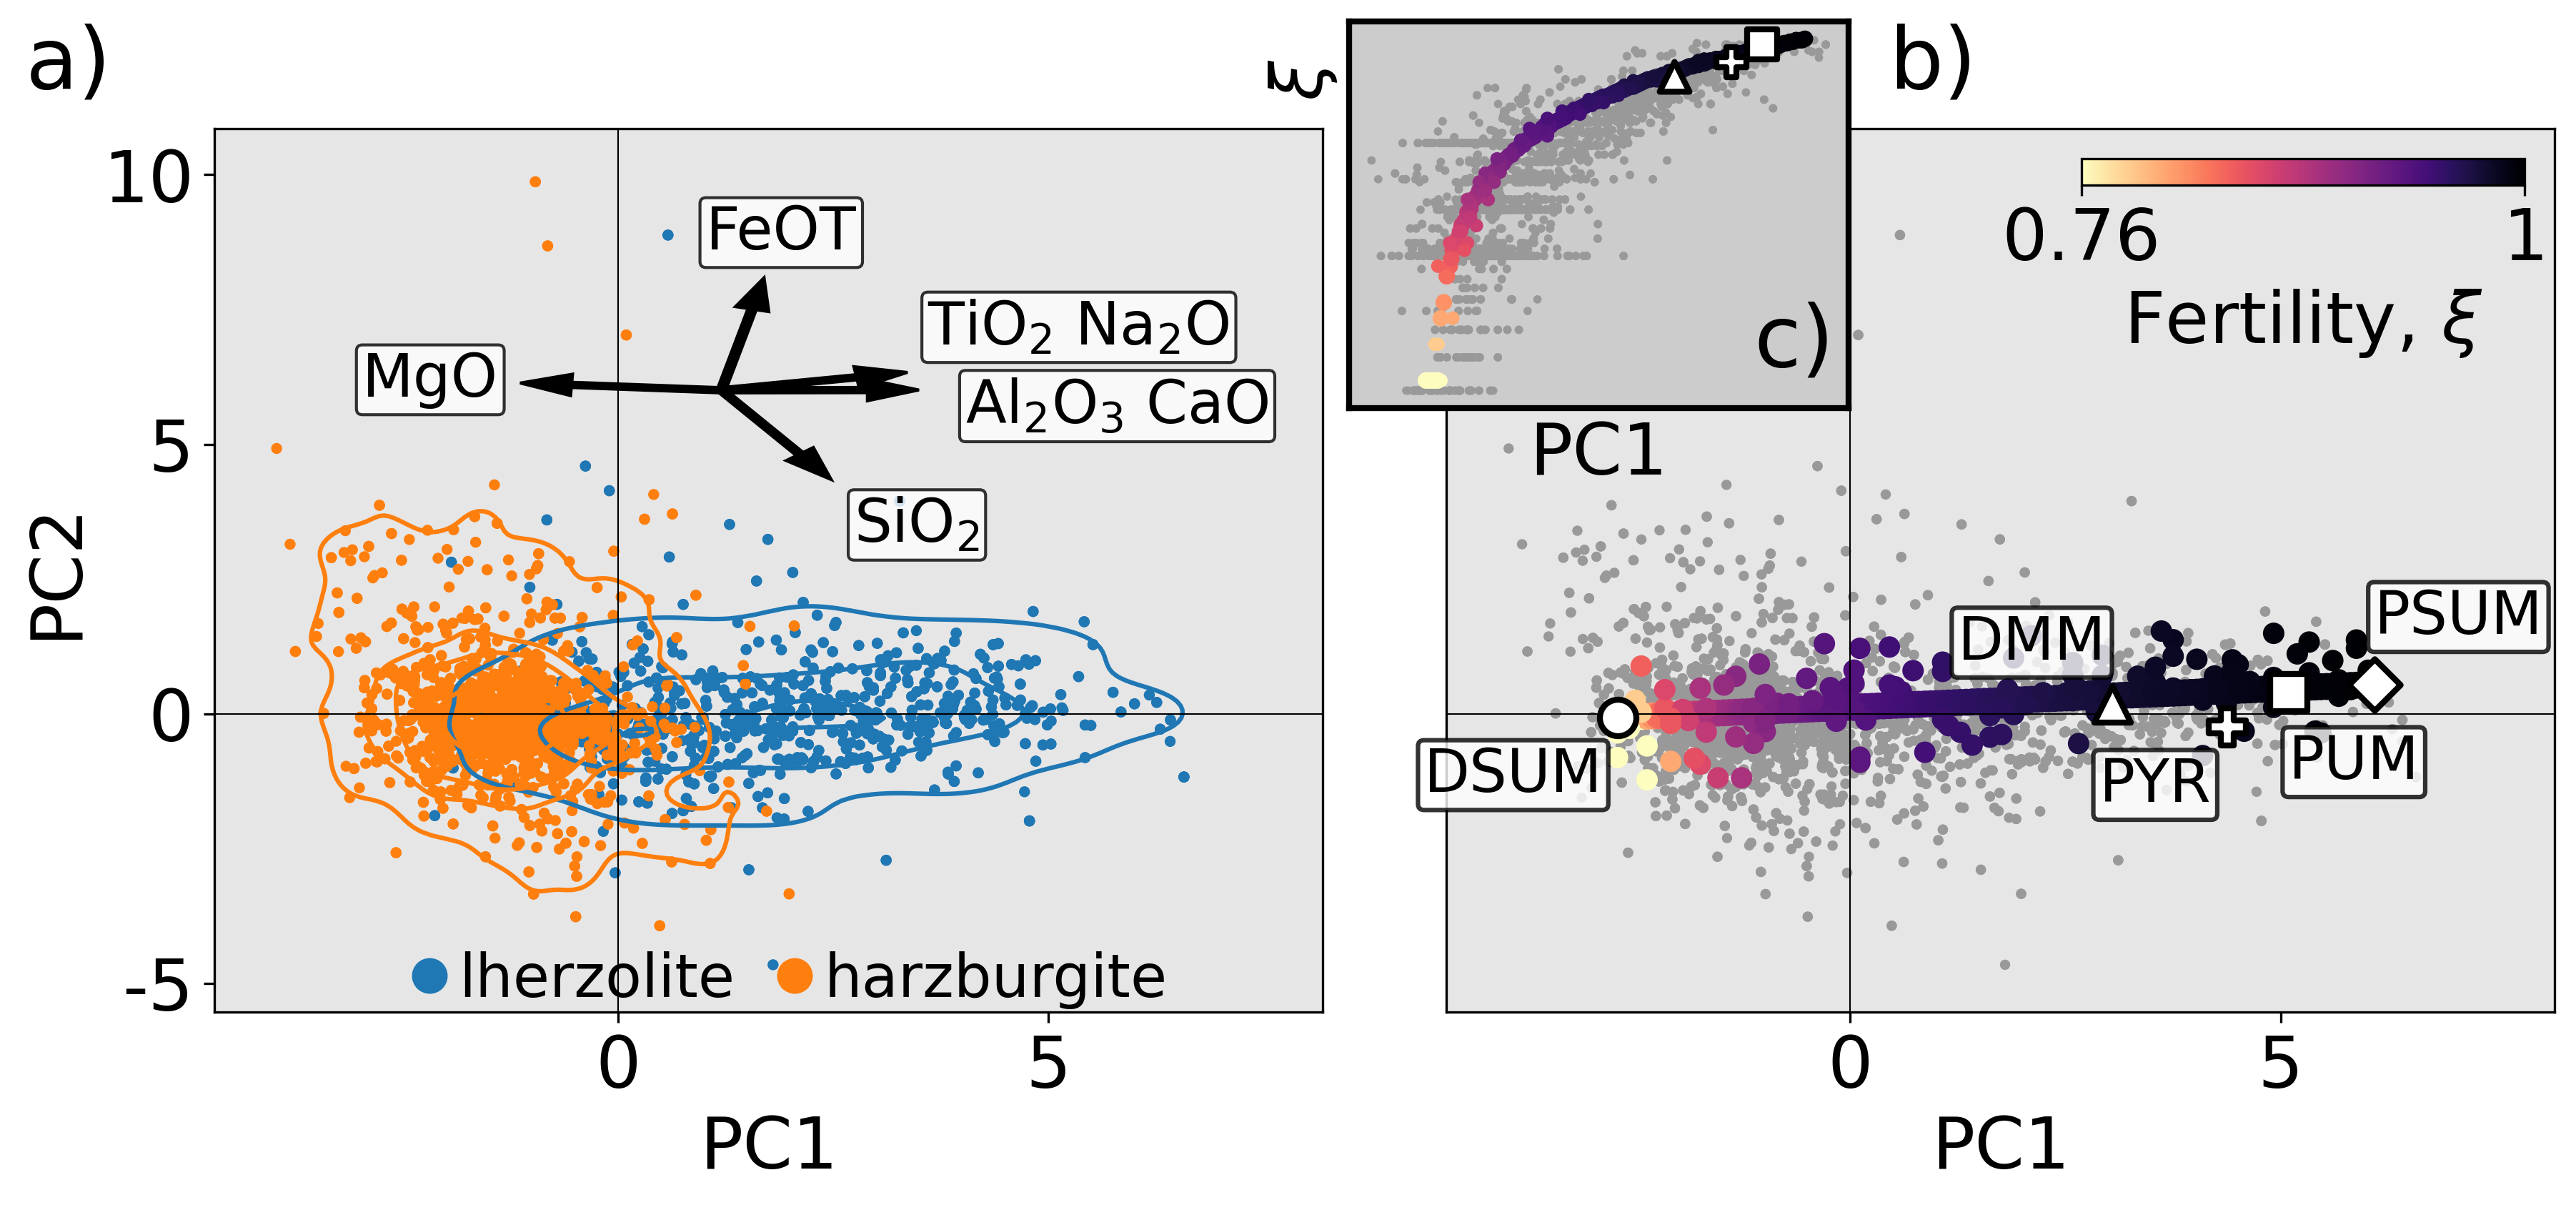
\includegraphics[width=1\linewidth,]{earthchem-mixing-array} 

}

\caption{PC1-PC2 diagrams showing the standardized geochemical dataset of natural peridotite samples (a) and a mixing array between hypothetical end-member mantle compositions Primitive Synthetic Upper Mantle (PSUM) and Depleted Synthetic Upper Mantle (DSUM, b). Black arrows in (a) indicate PCA loading vectors. Colored data points in (b) are the synthetic mantle compositions used to train RocMLMs, which were sampled independently from the natural peridotite samples (gray data points). The inset (c) shows how the Fertility Index (\(\xi\)) changes nonlinearly with PC1. DMM, PUM, and PYR are from Table \ref{tab:benchmark-samples}.}\label{fig:earthchem-mixing-array}
\end{figure}

The melting model in Equation \eqref{eq:shaw-melting} is oversimplified since it assumes: 1) melt is instantaneously removed from the source region, 2) \(D_0\) is constant, and 3) minerals melt in the same proportions that they exist in the source rock. It nevertheless provides an efficient parameterization of the variation in mantle composition as a function of melt extraction and addition. Equation \eqref{eq:shaw-melting} predicts that a Depleted MORB Mantle (DMM) composition is produced through a time-integrated 2.2\% melt extraction from a Primitive Upper Mantle (PUM) source (Table \ref{tab:benchmark-samples}). This result is consistent with the degree of depletion inferred from trace element patterns and mass balance constraints \citep[2-3\% melt removal from PUM,][]{workman2005}. We therefore consider \(\xi\) an adequate first-order proxy for describing the variations in bulk mantle composition used in our RocMLM training dataset. However, given that TiO\(_2\) concentrations are strongly affected by reactive melt transport \citep[e.g.,][]{le2007}, \(\xi\) may only be estimated for the average compositional trend as expressed in PC1-PC2 space, rather than on individual peridotite samples.

\begin{longtable}[]{@{}
  >{\raggedright\arraybackslash}p{(\columnwidth - 16\tabcolsep) * \real{0.0800}}
  >{\raggedleft\arraybackslash}p{(\columnwidth - 16\tabcolsep) * \real{0.1200}}
  >{\raggedleft\arraybackslash}p{(\columnwidth - 16\tabcolsep) * \real{0.1200}}
  >{\raggedleft\arraybackslash}p{(\columnwidth - 16\tabcolsep) * \real{0.1520}}
  >{\raggedleft\arraybackslash}p{(\columnwidth - 16\tabcolsep) * \real{0.1120}}
  >{\raggedleft\arraybackslash}p{(\columnwidth - 16\tabcolsep) * \real{0.1040}}
  >{\raggedleft\arraybackslash}p{(\columnwidth - 16\tabcolsep) * \real{0.1040}}
  >{\raggedleft\arraybackslash}p{(\columnwidth - 16\tabcolsep) * \real{0.1360}}
  >{\raggedleft\arraybackslash}p{(\columnwidth - 16\tabcolsep) * \real{0.0720}}@{}}
\caption{\label{tab:benchmark-samples} Hypothetical upper mantle end-member compositions. Columns with an asterisk are in wt.\%. Depleted MORB Mantle (DMM) is from \citet{workman2005}, Primitive Upper Mantle (PUM) is from \citet{sun1989}, and Pyrolite (PYR) is from \citet{green1979}. Primitive Synthetic Upper Mantle (PSUM) and Depleted Synthetic Upper Mantle (DSUM), are end-member compositions derived in this study.}\tabularnewline
\toprule\noalign{}
\begin{minipage}[b]{\linewidth}\raggedright
Sample
\end{minipage} & \begin{minipage}[b]{\linewidth}\raggedleft
SiO\(_2^{*}\)
\end{minipage} & \begin{minipage}[b]{\linewidth}\raggedleft
TiO\(_2^{*}\)
\end{minipage} & \begin{minipage}[b]{\linewidth}\raggedleft
Al\(_2\)O\(_3^{*}\)
\end{minipage} & \begin{minipage}[b]{\linewidth}\raggedleft
FeOT\(^{*}\)
\end{minipage} & \begin{minipage}[b]{\linewidth}\raggedleft
MgO\(^{*}\)
\end{minipage} & \begin{minipage}[b]{\linewidth}\raggedleft
CaO\(^{*}\)
\end{minipage} & \begin{minipage}[b]{\linewidth}\raggedleft
Na\(_2\)O\(^{*}\)
\end{minipage} & \begin{minipage}[b]{\linewidth}\raggedleft
\(\xi\)
\end{minipage} \\
\midrule\noalign{}
\endfirsthead
\toprule\noalign{}
\begin{minipage}[b]{\linewidth}\raggedright
Sample
\end{minipage} & \begin{minipage}[b]{\linewidth}\raggedleft
SiO\(_2^{*}\)
\end{minipage} & \begin{minipage}[b]{\linewidth}\raggedleft
TiO\(_2^{*}\)
\end{minipage} & \begin{minipage}[b]{\linewidth}\raggedleft
Al\(_2\)O\(_3^{*}\)
\end{minipage} & \begin{minipage}[b]{\linewidth}\raggedleft
FeOT\(^{*}\)
\end{minipage} & \begin{minipage}[b]{\linewidth}\raggedleft
MgO\(^{*}\)
\end{minipage} & \begin{minipage}[b]{\linewidth}\raggedleft
CaO\(^{*}\)
\end{minipage} & \begin{minipage}[b]{\linewidth}\raggedleft
Na\(_2\)O\(^{*}\)
\end{minipage} & \begin{minipage}[b]{\linewidth}\raggedleft
\(\xi\)
\end{minipage} \\
\midrule\noalign{}
\endhead
\bottomrule\noalign{}
\endlastfoot
DSUM & 44.1 & 0.0012 & 0.261 & 7.96 & 47.4 & 0.22 & 0.042 & 0.764 \\
DMM & 44.7 & 0.13 & 3.98 & 8.18 & 38.7 & 3.17 & 0.13 & 0.974 \\
PYR & 45 & 0.16 & 4.4 & 7.6 & 38.8 & 3.4 & 0.34 & 0.984 \\
PUM & 44.9 & 0.2 & 4.44 & 8.03 & 37.7 & 3.54 & 0.36 & 0.996 \\
PSUM & 46.2 & 0.216 & 4.88 & 8.88 & 35.2 & 4.34 & 0.33 & 1 \\
\end{longtable}

\subsection{Generating RocMLM Training Data}\label{sec:generate-training-data}

We used the GFEM program Perple\_X \citep[version 7.0.9,][]{connolly2009} to generate RocMLM training data across PT conditions as described in Section \ref{sec:pt-conditions} and synthetic bulk mantle compositions as described in Section \ref{sec:bulk-rock-compositions}. The Perple\_X calculations were constrained to the Na\(_2\)O-CaO-FeO-MgO-Al\(_2\)O\(_3\)-SiO\(_2\) (NCFMAS) chemical system to comply with the thermodynamic data and solution models of \citet{stixrude2022}. The \citet{stixrude2022} dataset (stx21ver.dat) was used because our initial tests with alternative thermodynamic datasets \citep[hp02ver.dat and hp633ver.dat,][]{connolly2002, holland2001, holland2018} failed to reproduce the seismic wave velocities of geophysical reference models \citep[PREM and STW105,][]{dziewonski1981, kustowski2008} with sufficient accuracy because these datasets lack a parametrization of the shear modulii of the minerals phases. Note that our Perple\_X calculations ignored TiO\(_2\), which was initially included to define \(\xi\) and derive synthetic bulk mantle compositions. Despite being measured as a major oxide component, the average TiO\(_2\) content of our standardized samples is 0.05 ± 0.1 wt.\% (2\(\sigma\), Table \ref{tab:earthchem-counts}). Such small concentrations of TiO\(_2\) may safely be ignored in phase relation calculations with negligible effects on the RocMLM training dataset.

The Perple\_X models used to generate the present RocMLM training database included equations of state for solution phases: olivine, plagioclase, spinel, clinopyroxene, wadsleyite, ringwoodite, perovskite, ferropericlase, high-pressure C2/c pyroxene, orthopyroxene, akimotoite, post-perovskite, Ca-ferrite, garnet, and Na-Al phase. Melt was not considered due to the absence of melt models in the \citet{stixrude2022} dataset, but may be considered in future versions of training datasets if the elastic parameters in hp02ver.dat are corrected. Once configured, Perple\_X generated RocMLM training data (density, as well as P- and S-wave seismic velocities) by minimizing the total Gibbs Free Energy of a multicomponent multiphase thermodynamic system at fixed PTX conditions \citep{gibbs1878, spear1993}. The reader is referred to \citet{connolly2009} and \citet{riel2022} for a complete description of the GFEM problem.

In principle, applying identical sets of solution phase models, thermodynamic data, and bulk compositions will define identical Gibbs Free Energy hyperplanes. This implies that any GFEM algorithm should converge on identical phase relations. Thus, although this study uses Perple\_X exclusively, an identical set of training data can be generated by applying the procedures outlined above to other GFEM programs. Note that RocMLM capabilities and performance are primarily dependent on the size and the range of PTX conditions of the training dataset, not on the choice of GFEM algorithm.

\subsection{Training RocMLMs}\label{sec:train-rocmlms}

RocMLM training data were preprocessed using the following procedure. First, two-dimensional grids of rock properties (``pseudosections'') calculated by Perple\_X were stacked into a three-dimensional array, \(Z\) = \((z_{1,1,1}, \ldots,z_{n,w,w})\), where \(w\) = 128 is the resolution of the PT grid and \(n\) = 128 is the number of random synthetic bulk mantle compositions represented by a \(\xi\) value. \(Z\) was flattened into arrays of training features (PT and \(\xi\)), \(X\) = \((x_{1,1,1}, \ldots, x_{v,v,v})\), and training targets (density, Vp, and Vs), \(y\) = \((y_{1,1,1}, \ldots, y_{v,v,v})\), where \(v\) = \(n \cdot w^2\) = 128\(^3\) is the total number of training examples. Following common practice, \(X\) and \(y\) were scaled using ``z-score normalization'' before training.

The preprocessed training data were then fit with three different nonlinear regression algorithms (Decision Tree: DT, k-Neighbors: KN, and Neural Networks: NN) from the scikit-learn python library \citep{scikit2011}. Each regression algorithm was tuned with a grid search approach, where a performance score (RMSE) was evaluated over all hyperparameter combinations relevant to the particular regression algorithm (Table \ref{tab:rocmlm-config}). The set of hyperparameters that produced the best score (lowest RMSE) was used to train the RocMLM.

\begin{longtable}[]{@{}
  >{\raggedright\arraybackslash}p{(\columnwidth - 6\tabcolsep) * \real{0.1098}}
  >{\raggedright\arraybackslash}p{(\columnwidth - 6\tabcolsep) * \real{0.2439}}
  >{\raggedright\arraybackslash}p{(\columnwidth - 6\tabcolsep) * \real{0.5366}}
  >{\raggedright\arraybackslash}p{(\columnwidth - 6\tabcolsep) * \real{0.1098}}@{}}
\caption{\label{tab:rocmlm-config} RocMLM configuration. Hyperparameter values in parentheses are tested sequentially by a cross-validation grid search algorithm and the best set of hyperparameters is chosen by the lowest RMSE. Hyperparameters that are not shown use default values (see regression model documentation on scikit-learn.org).}\tabularnewline
\toprule\noalign{}
\begin{minipage}[b]{\linewidth}\raggedright
Model
\end{minipage} & \begin{minipage}[b]{\linewidth}\raggedright
Hyperparameter
\end{minipage} & \begin{minipage}[b]{\linewidth}\raggedright
Value
\end{minipage} & \begin{minipage}[b]{\linewidth}\raggedright
Tuned
\end{minipage} \\
\midrule\noalign{}
\endfirsthead
\toprule\noalign{}
\begin{minipage}[b]{\linewidth}\raggedright
Model
\end{minipage} & \begin{minipage}[b]{\linewidth}\raggedright
Hyperparameter
\end{minipage} & \begin{minipage}[b]{\linewidth}\raggedright
Value
\end{minipage} & \begin{minipage}[b]{\linewidth}\raggedright
Tuned
\end{minipage} \\
\midrule\noalign{}
\endhead
\bottomrule\noalign{}
\endlastfoot
DT & splitter & (best, random) & tuned \\
& max features & (1, 2, 3) & tuned \\
& min samples leaf & (1, 2, 3) & tuned \\
& min samples split & (2, 4, 6) & tuned \\
KN & n neighbors & (2, 4, 8) & tuned \\
& weights & (uniform, distance) & tuned \\
NN1 & hidden layer sizes & (8, 16, 32) & tuned \\
NN2 & hidden layer sizes & ({[}16, 16{]}, {[}32, 16{]}, {[}32, 32{]}) & tuned \\
NN3 & hidden layer sizes & ({[}32, 16, 16{]}, {[}32, 32, 16{]}, {[}32, 32, 32{]}) & tuned \\
NN(all) & learning rate & (0.001, 0.005, 0.001) & tuned \\
& batch size & 20\% & fixed \\
& max epochs & 100 & fixed \\
\end{longtable}

\subsection{Evaluating RocMLM Accuracy and Performance}\label{sec:evaluate-rocmlms}

\citet{connolly2016} estimated the uncertainties of Vp and Vs to be on the order of 3--5\% within the same thermodynamic framework used to generate RocMLM training data \citep{stixrude2005}. We can therefore consider the base-uncertainty of RocMLM predictions to be 3--5\%. RocMLM predictions must also account for additional uncertainties that are introduced during RocMLM training (i.e., the variance of residuals between RocMLM predictions and targets), which are about 2\% for NN1 and \textless{} 1\% for DT, KN, and NN3. Assuming the lowest-uncertainty models (DT, KN, NN3) would be preferred for geodynamic applications, we ignore the small variances introduced during training (\textless{} 1\%) and evaluate the total RocMLM prediction uncertainties to be on the same order as the base GFEM uncertainty (3--5\%) after \citet{connolly2016}.

RocMLM accuracy (in terms of RMSE) was evaluated by: 1) testing RocMLMs on a separate validation dataset to determine the generalization capacity of RocMLMs to unseen mantle conditions (internal accuracy), and 2) comparing RocMLMs predictions with geophysical reference models PREM and STW105 (external accuracy). The first test evaluates the degree to which RocMLMs can reproduce GFEM predictions. The second test evaluates the degree to which the ``true data'' used for RocMLM training reproduces the phase transitions actually observed in Earth's upper mantle, which depend on the thermodynamic data, GFEM algorithm, and parameterization used to describe the composition of mantle rocks (i.e., \(\xi\)).

The validation dataset was generated by Perple\_X in the same manner as the training dataset, but shifted by one-half step (in the positive PT directions) so that RocMLM predictions could be evaluated at completely independent PT conditions. RocMLM performance was evaluated by: 1) measuring single-point prediction times (execution speed), and 2) scaling execution speed by RocMLM file size (disk space) to account for information compression (model efficiency).

The number of PT points and synthetic bulk mantle compositions used for generating training data were varied from 8 to 128 (2\(^{11}\)--2\(^{21}\) total training examples) to test the sensitivity of RocMLM accuracy and performance with respect to the size (``capacity'') and composition of the training dataset. The same sets of training data were also used to evaluate single-point execution speed using a common Lookup Table approach, where a cubic spline interpolation was applied to the training dataset and rock properties were evaluated at arbitrary PTX conditions. Prediction accuracy and performance were measured in a consistent manner so that direct comparisons could be made between RocMLMs, Lookup Tables, and GFEM programs.

\section{Results}\label{sec:results}

\subsection{RocMLM Accuracy}\label{sec:rocmlms-accuracy}

The following examples of Decision Tree (DT, Figure \ref{fig:image12-PUM-DT}), single-layer Neural Network (NN1, Figure \ref{fig:image12-PUM-NN1}), and three-layer Neural Network (NN3, Figure \ref{fig:image12-PUM-NN3}) models demonstrate how different regression algorithms ultimately influence the accuracy of RocMLM predictions (see Supplementary Information for all regression algorithms).

DT predictions are practically indistinguishable from that of Perple\_X, indicating a nearly-perfect mapping of the validation dataset by the DT algorithm (RMSE for density: 0.01 g/cm\(^3\), Vp and Vs: 0.02 km/s, Figure \ref{fig:image12-PUM-DT}). Absolute differences between Perple\_X and DT predictions (residuals) are broadly dispersed and approach zero in most regions of PT space. Some concentrations of residuals exist near phase transitions, but are subtle and discontinuous (Figure \ref{fig:image12-PUM-DT}g--i).

In contrast, NN1 predictions are notably smoother than Perple\_X (Figure \ref{fig:image12-PUM-NN1}), with higher errors (RMSE for density: 0.02 g/cm\(^3\), Vp: 0.06 km/s, Vs: 0.05 km/s) that indicate an inability to resolve sharp gradients in physical properties when using a single-layer Neural Network with a small to moderate amount of neurons. This is evident by the NN1 residuals, which are systematically concentrated near phase transitions (Figure \ref{fig:image12-PUM-NN1}g--i). NN1 profiles display relatively weak discontinuities with gradual changes in physical properties across the olivine → wadsleyite and ringwoodite → bridgmanite + ferropericlase transitions (Figure \ref{fig:image12-PUM-NN1}j--l), and phase transformations within the MTZ are virtually absent compared to DT and NN3 profiles. While NN1 predictions do not reproduce the validation dataset or geophysical profiles with the highest accuracy, deeper (and/or wider) NN architectures with more hidden-layers (e.g., NN3) are more capable (Figure \ref{fig:image12-PUM-NN3}). NN3 predictions fit the validation dataset and resolve discontinuities in geophysical profiles with nearly equivalent accuracy as DT and KN algorithms (compare profiles in Supplementary Information).

Comparing density, Vp, and Vs depth profiles predicted by RocMLMs (for an average mid-ocean ridge-like geotherm with a mantle potential temperature of 1573 K) with PREM and STW105 reveals relatively low errors (density: ≤ 0.08 g/cm\(^3\), Vp: ≤ 0.26 km/s, Vs: ≤ 0.14 km/s) and high correlations (R\(^2\) ≥ 0.94) that indicate good agreement between seismically-derived profiles and thermodynamic predictions, irrespective of regression algorithm (compare profiles in the Supplementary Information). The largest deviations between RocMLM profiles, PREM, and STW105 fall within two regions: 1) between 1--8 GPa, and 2) at the base of the MTZ (Figures \ref{fig:image12-PUM-DT}--\ref{fig:image12-PUM-NN3}j--l). At pressures lower than 5 GPa, the divergence between RocMLM profiles and seismically-derived profiles may be explained by the low resolution of the 1D geophysical profiles relative to the extreme spatial variability in composition and geotherms on Earth. Tests using an average continental geotherm to calculate RocMLM profiles results in less divergence between RocMLM profiles and PREM at \textless{} 5 GPa compared to the mid-ocean ridge-like geotherms used to build the profiles presented in Figures \ref{fig:image12-PUM-DT}--\ref{fig:image12-PUM-NN3}. At pressures between 5--8 GPa, the two geophysical models show a discrepancy: PREM contains a discontinuity, especially in seismic velocities, while STW105 has a gradual and continuous increase. RocMLM profiles between 5--8 GPa are more similar to STW105, which does not map any discontinuities until the olivine → wadsleyite transition at 410 km depth (Figures \ref{fig:image12-PUM-DT}--\ref{fig:image12-PUM-NN3}j--l).

Within the MTZ, DT and NN3 profiles predict intermediate discontinuities, while PREM and STW105 are gradual and continuous (Figures \ref{fig:image12-PUM-DT},\ref{fig:image12-PUM-NN3}g--i). As expected, comparing RocMLM profiles for different geotherms shows that the choice of a mantle potential temperature leads to contrasting predictions of: 1) the overall evolution of rock properties with depth, and 2) the depths, magnitudes, and sharpness of phase transitions within the MTZ (Figures \ref{fig:image12-PUM-DT}--\ref{fig:image12-PUM-NN3}g--i). RocMLM profiles show, similarly to those directly derived from the Perple\_X calculation, temperature-sensitive discontinuities at the olivine → wadsleyite and wadsleyite → ringwoodite transitions, but a rather temperature insensitive ringwoodite → bridgmanite + ferropericlase transition (Figures \ref{fig:image12-PUM-DT}--\ref{fig:image12-PUM-NN3}g--i). This can be explained by differences in Clapeyron slopes modeled by the \citet{stixrude2022} dataset.



\begin{figure}[htbp]

{\centering 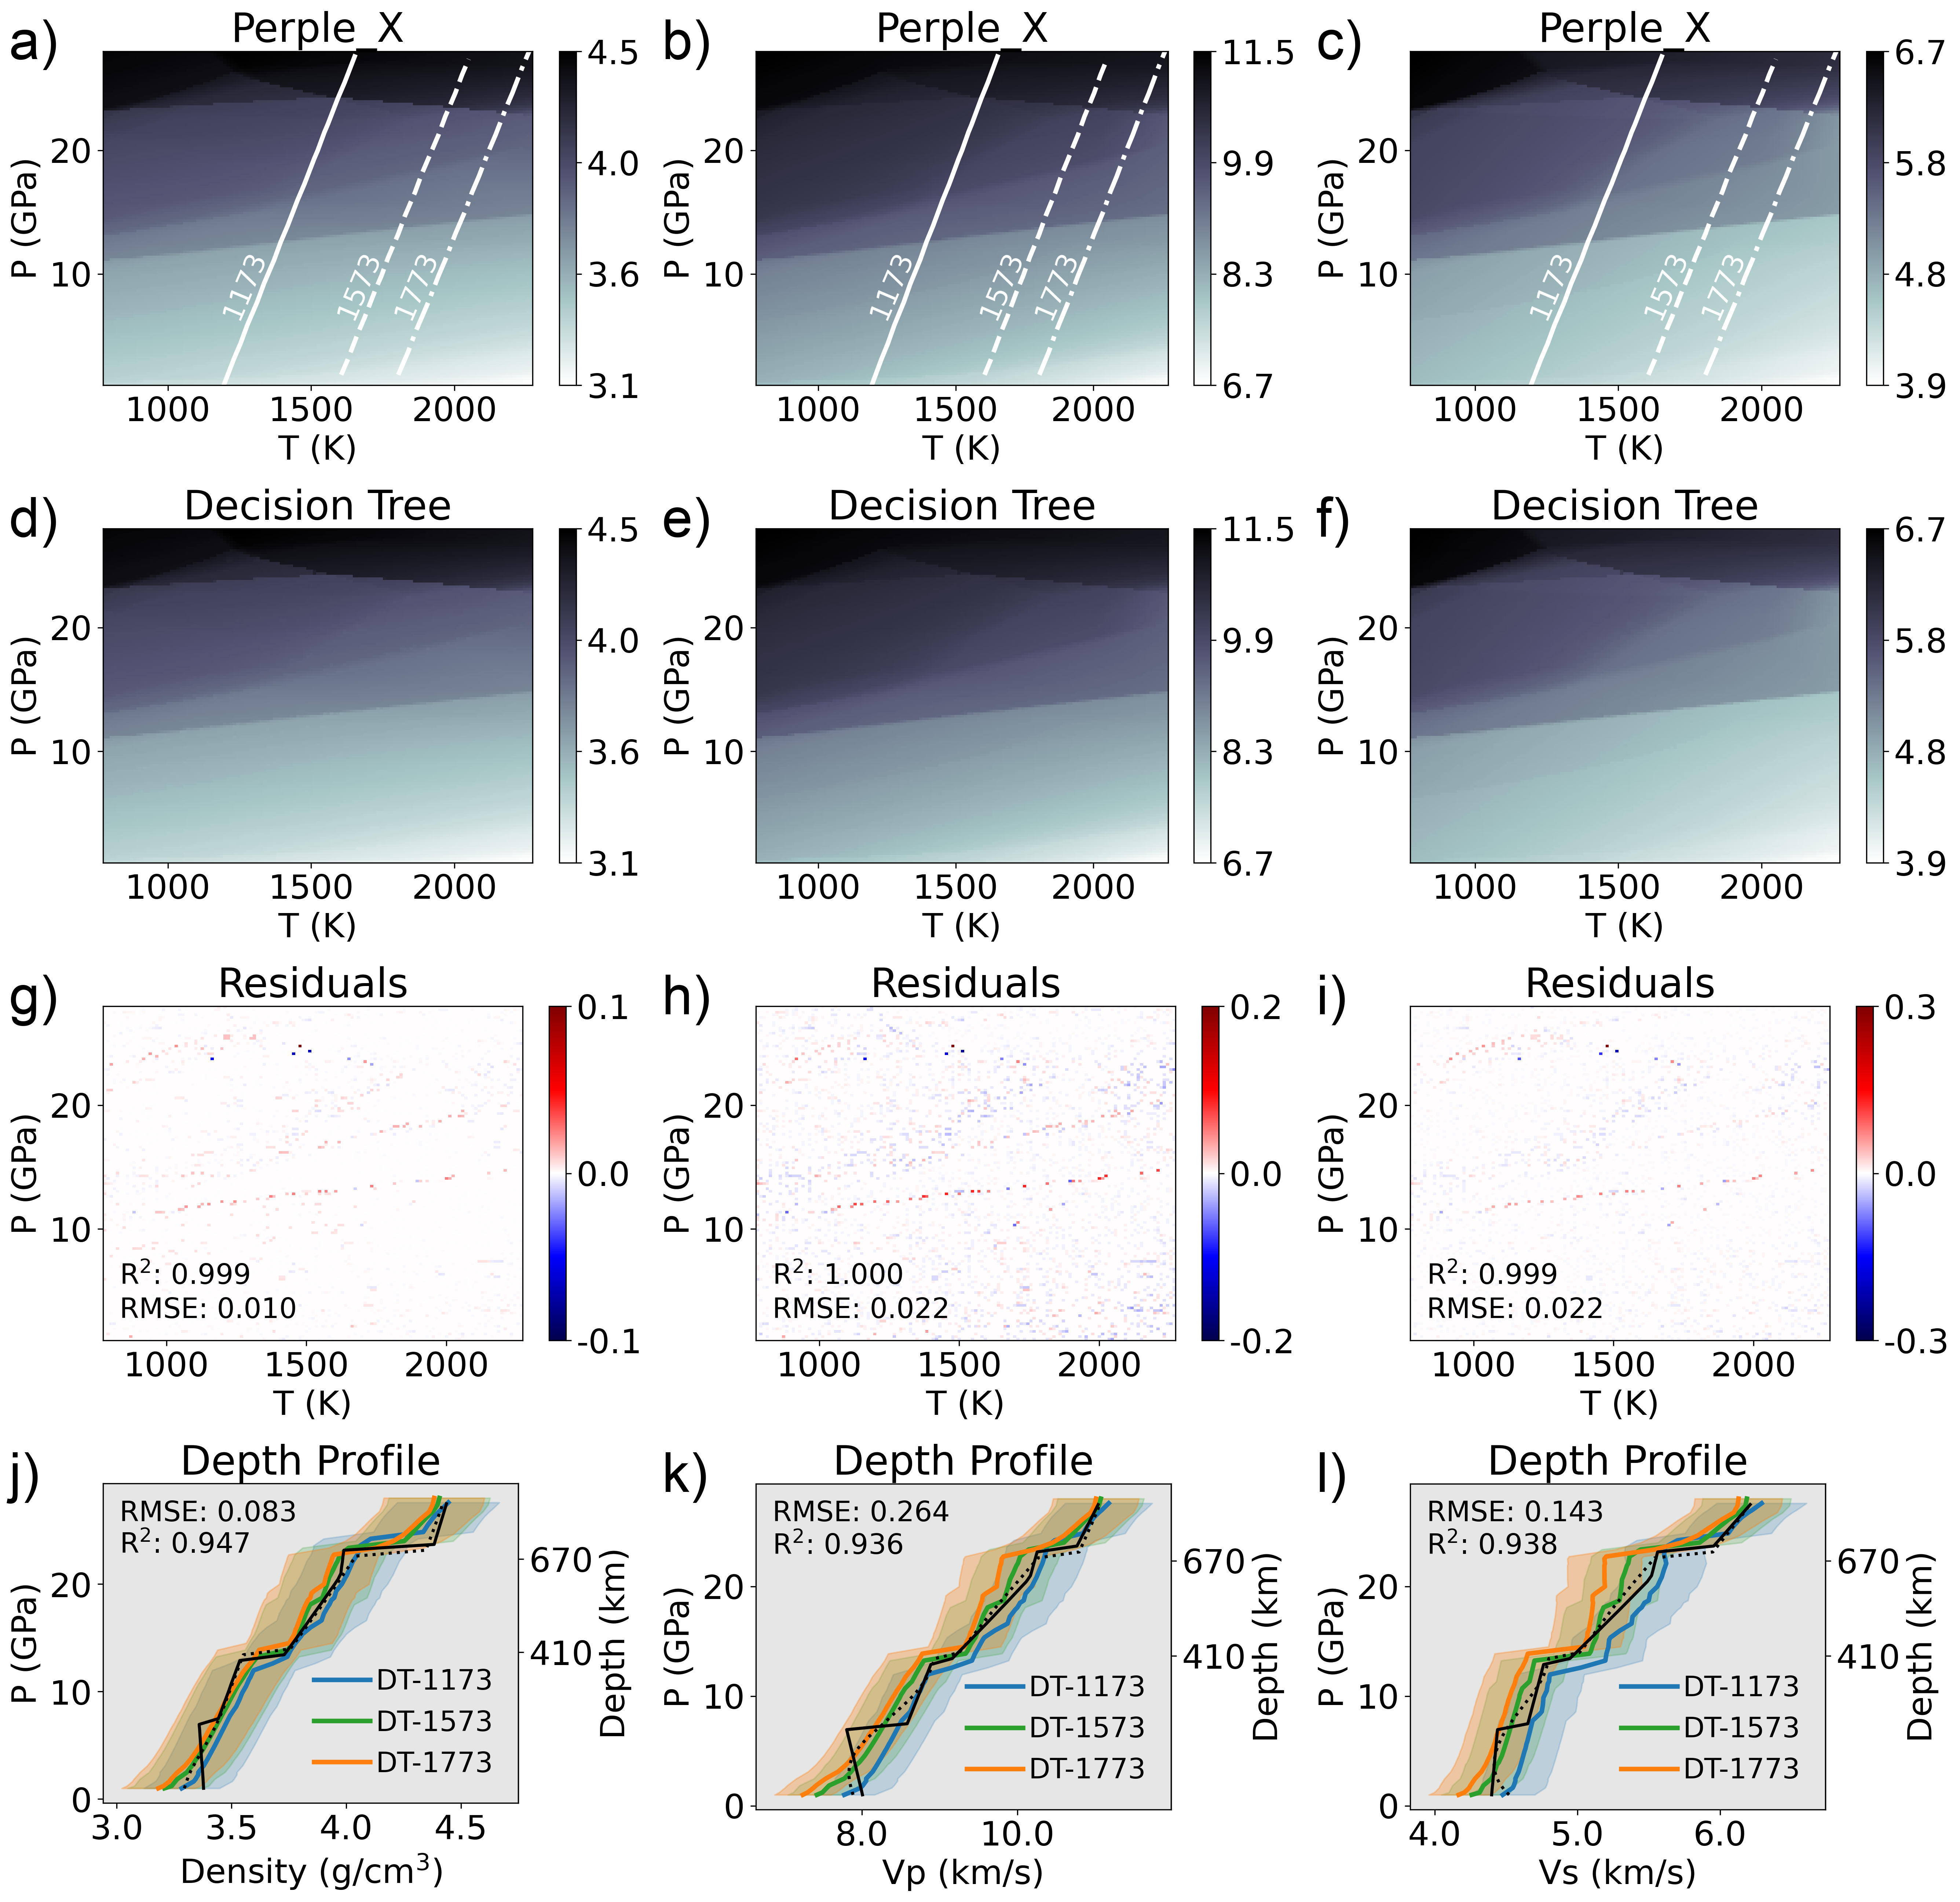
\includegraphics[width=1\linewidth,]{image12-PUM-DT} 

}

\caption{PT diagrams showing density (left column, g/cm\(^3\)), Vp (middle column, km/s), and Vs (right column, km/s) predictions from a Perple\_X model with a PUM bulk composition (a--c), a Decision Tree RocMLM (d--f), and absolute differences between Perple\_X and DT (g--i) measured on the validation dataset. Depth profiles (j--l) compare Perple\_X and DT predictions extracted along a 0.5 K/km adiabat with different mantle potential temperatures (white lines) with reference models PREM \citep[solid black line,][]{dziewonski1981} and STW105 \citep[dotted black line,][]{kustowski2008}. The RMSE in (j--l) indicates the measured differences between DT-1573 and PREM. Colored ribbons indicate 5\% uncertainty in RocMLM predictions.}\label{fig:image12-PUM-DT}
\end{figure}



\begin{figure}[htbp]

{\centering 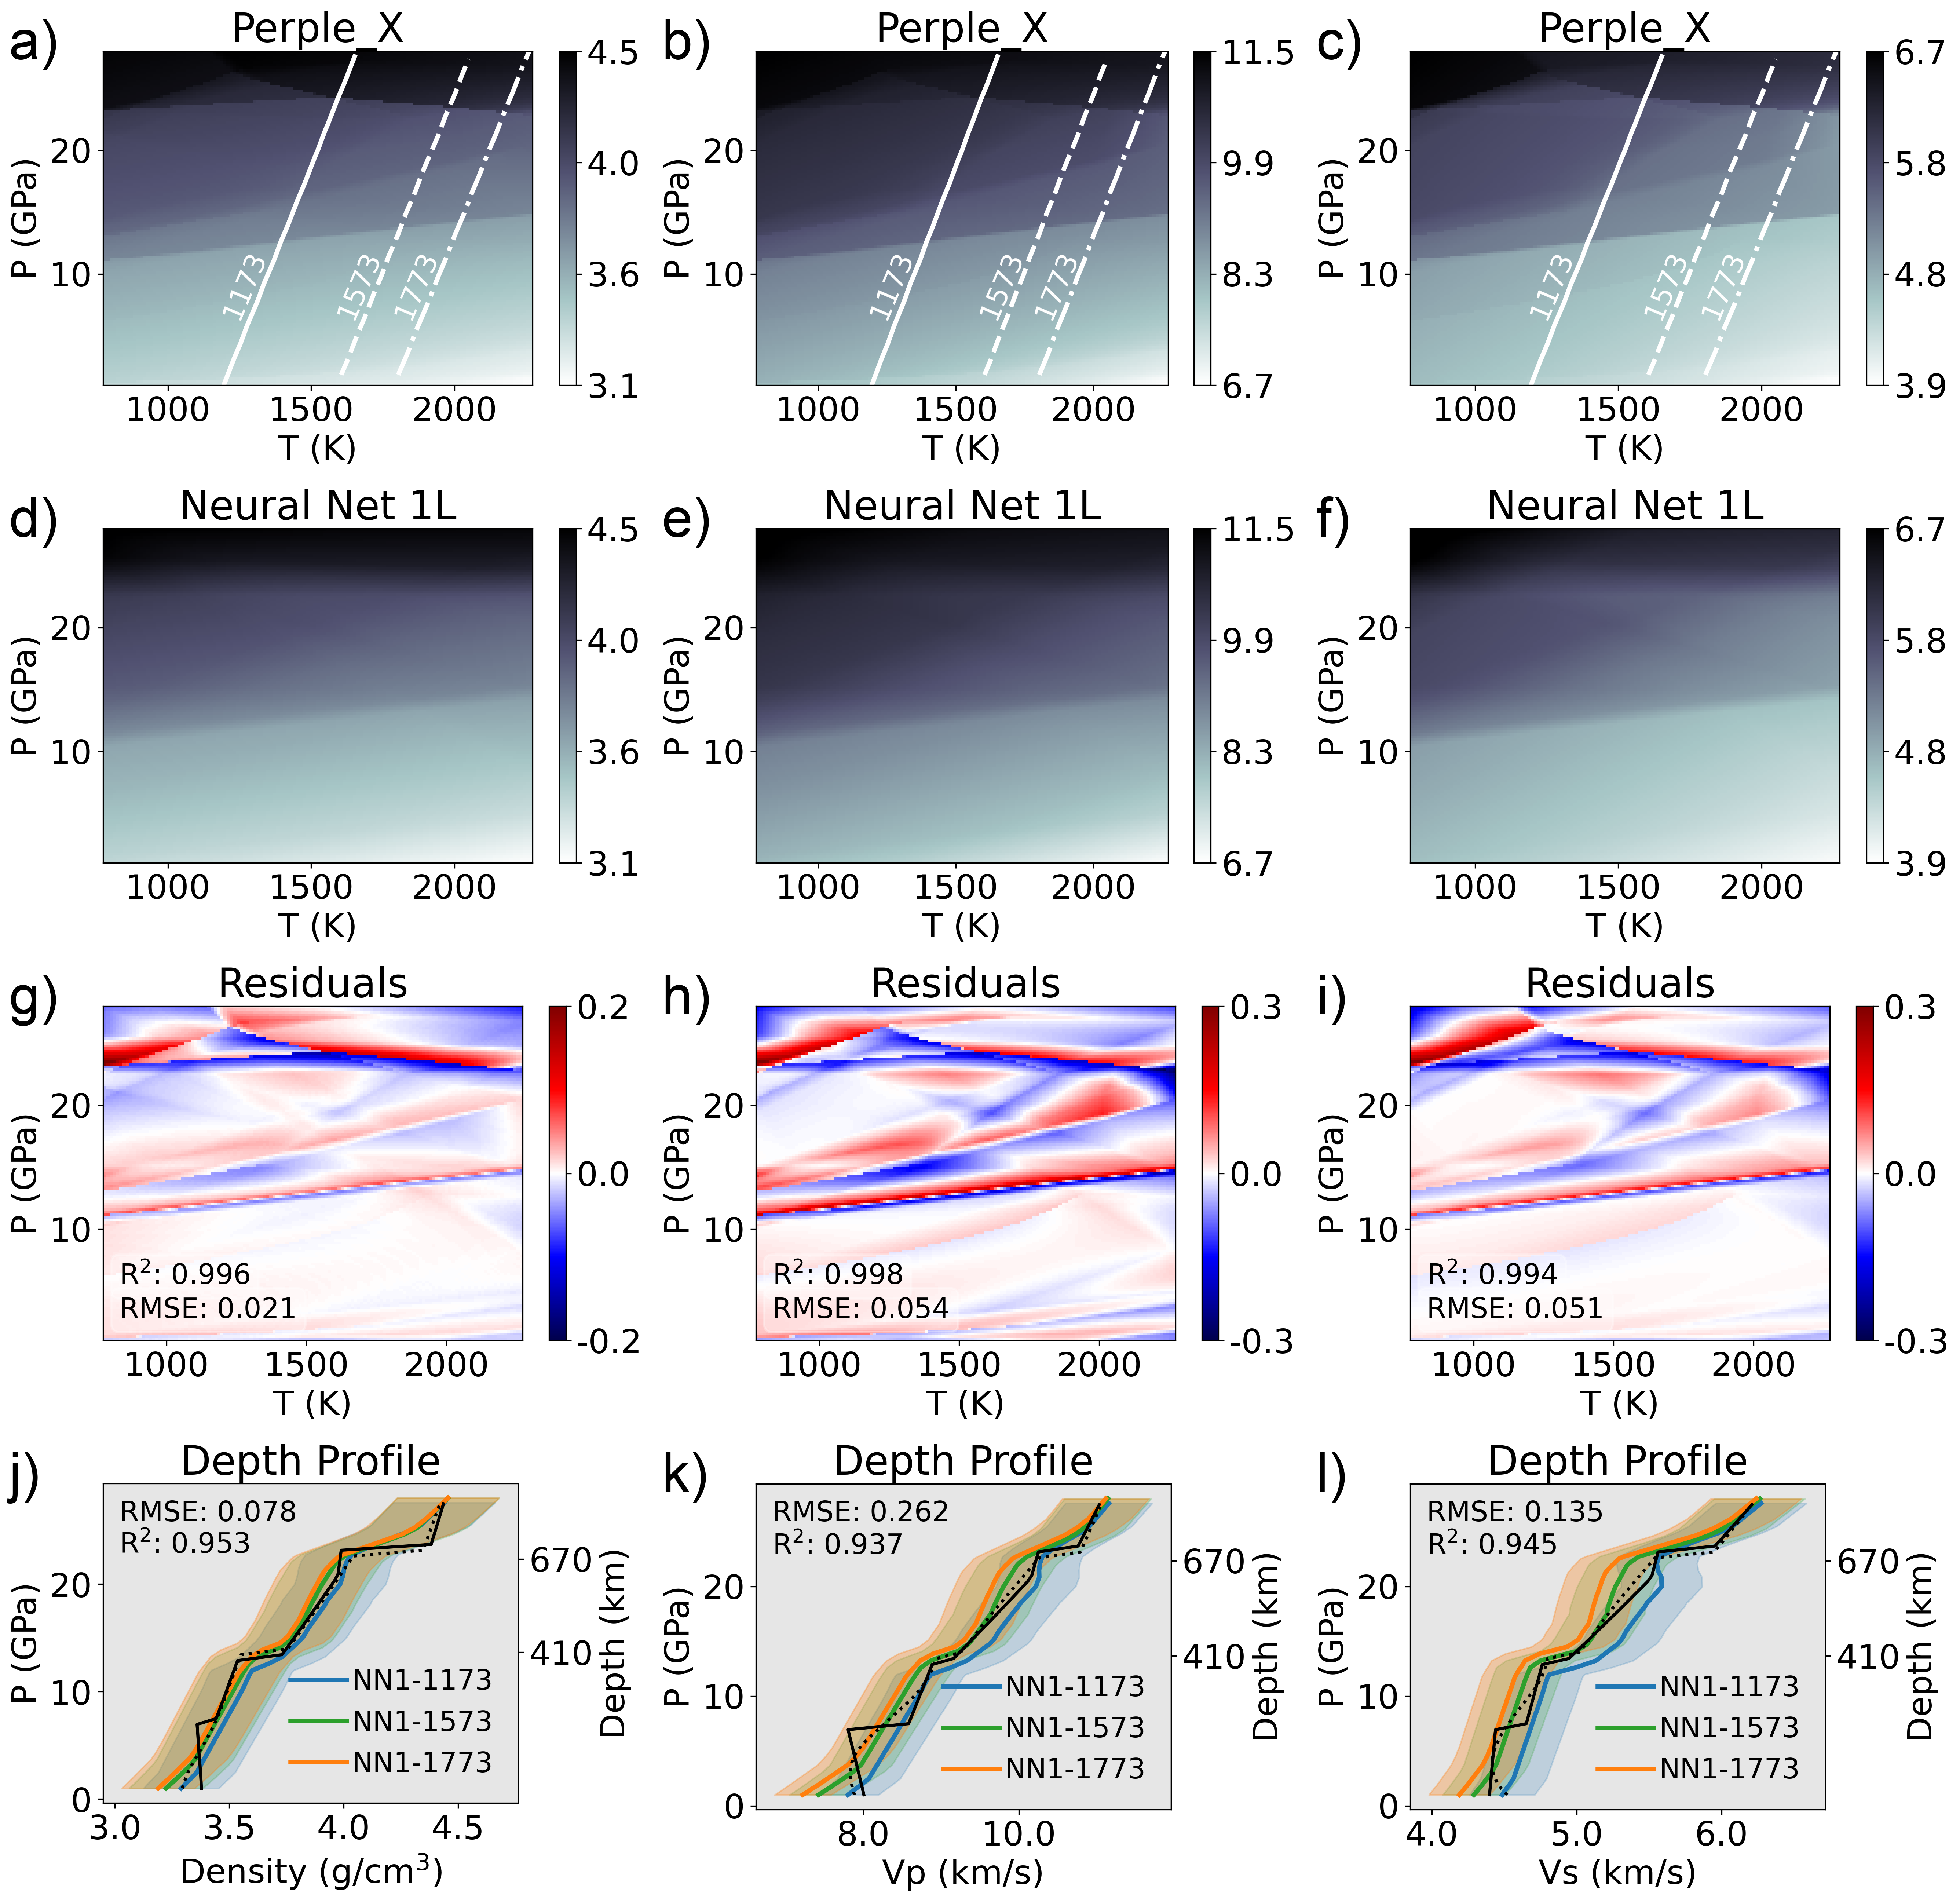
\includegraphics[width=1\linewidth,]{image12-PUM-NN1} 

}

\caption{PT diagrams showing density (left column, g/cm\(^3\)), Vp (middle column, km/s), and Vs (right column, km/s) predictions from a Perple\_X model with a PUM bulk composition (a--c), a single-layer Neural Network RocMLM (d--f), and absolute differences between Perple\_X and NN1 (g--i) measured on the validation dataset. Other legend details are the same as in Figure 3.}\label{fig:image12-PUM-NN1}
\end{figure}



\begin{figure}[htbp]

{\centering 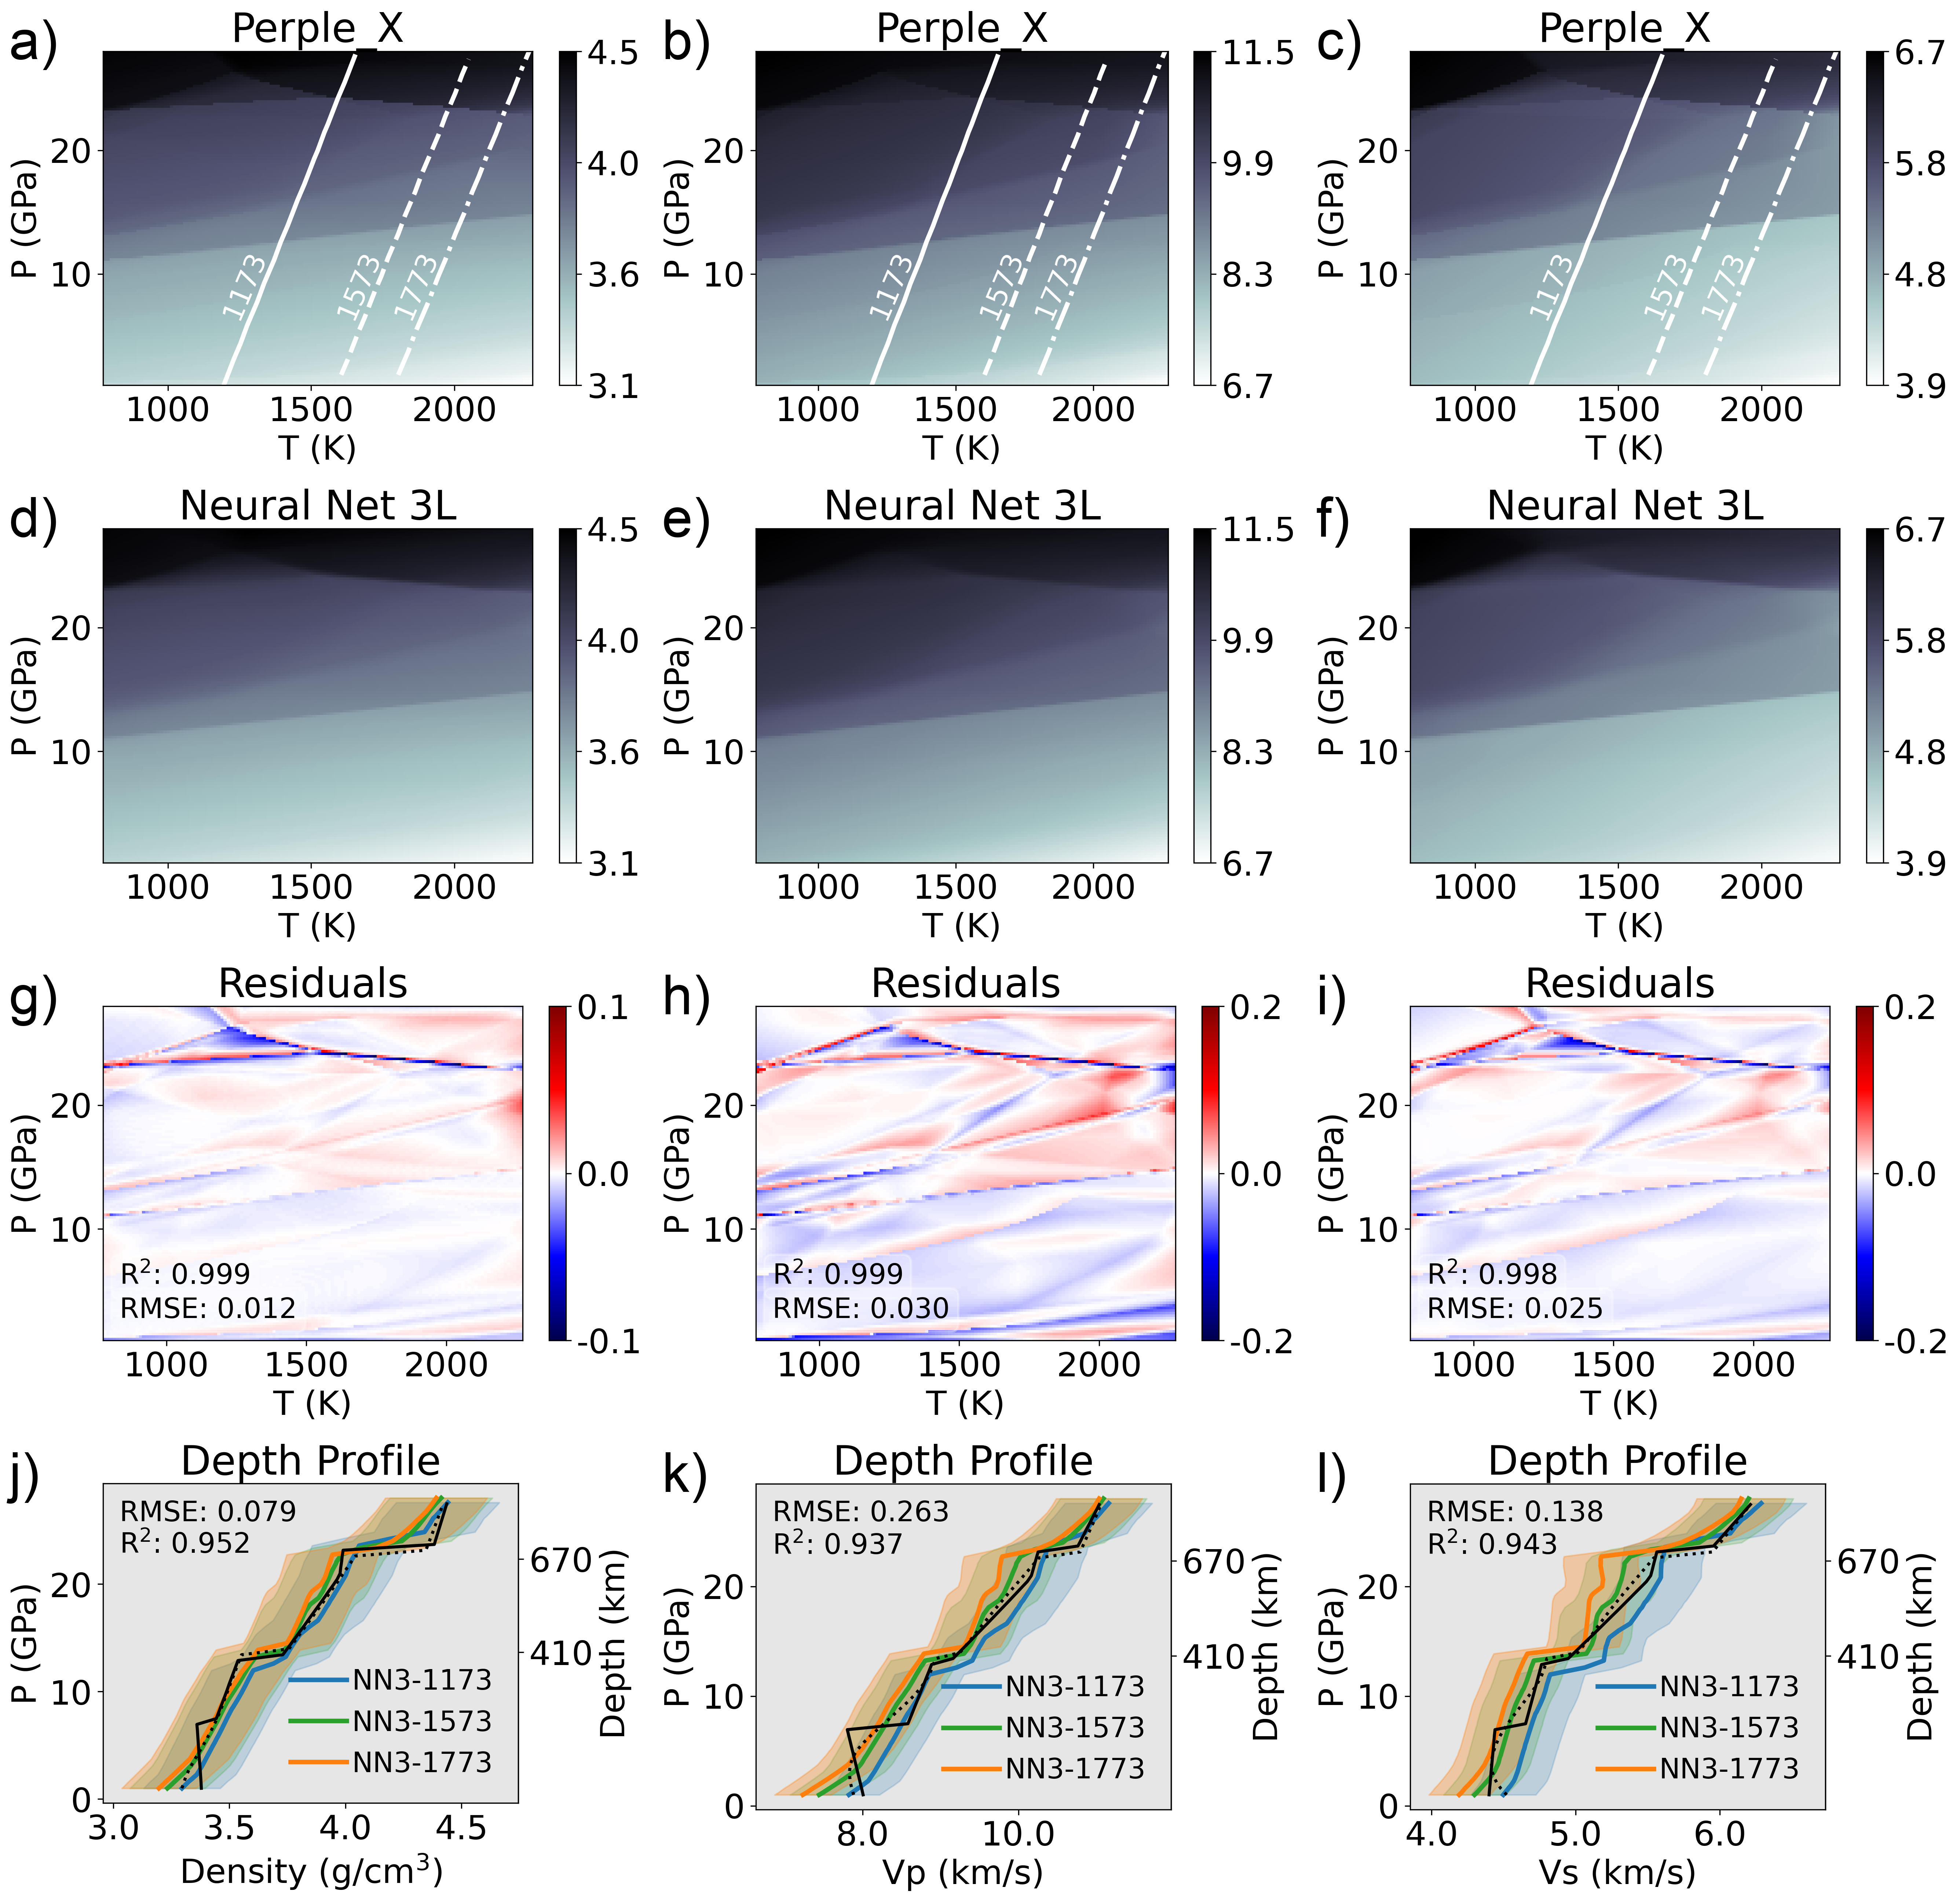
\includegraphics[width=1\linewidth,]{image12-PUM-NN3} 

}

\caption{PT diagrams showing density (left column, g/cm\(^3\)), Vp (middle column, km/s), and Vs (right column, km/s) predictions from a Perple\_X model with a PUM bulk composition (a--c), a three-layer Neural Network RocMLM (d--f), and absolute differences between Perple\_X and NN3 (g--i) measured on the validation dataset. Other legend details are the same as in Figure 3.}\label{fig:image12-PUM-NN3}
\end{figure}

\subsection{RocMLM Performance}\label{sec:rocmlm-performance-and-efficiency}

We now compare RocMLM performance to two other tools classically used to predict the variations of physical properties of mantle rocks in geodynamic models: GFEM programs and Lookup Tables. Note that RocMLM, GFEM, and Lookup Table performance is platform specific. Running analogous implementations with other programming languages and/or on alternative computer hardware will differ from the results presented here. All computations in this study were made using CPUs of a Macbook Pro (2022; M2 chip) with macOS 13.4 and using Python 3.11.4. All performance metrics were evaluated with a single CPU core.

Figure \ref{fig:rocmlm-performance} shows how execution speed, efficiency, and accuracy scale with the capacity of Lookup Tables and RocMLMs. Here, ``capacity'' refers to the number of scalar values stored by Lookup Tables, or alternatively, the number of pseudosection PTX points ``learned'' by RocMLMs. Thus, ``capacity'' is intended to convey and compare the breadth of petrological ``knowledge'', or predictive capabilities, of Lookup Tables and RocMLMs. Within the same context, the notion of ``capacity'' is irrelevant for GFEM programs. Rather, GFEM performance primarily scales with the number of chemical components, phase solutions, and size of the compositional space defined by the user, as well as automatic grid refinement settings and other user-defined configuration options.

GFEM performance is reported using the range of average execution speeds (4--228 ms) and efficiencies (60--3138 ms\(\cdot\)Mb) that we measured while generating our RocMLM training datasets as described in Section \ref{sec:generate-training-data}. To demonstrate the sensitivity of GFEM performance to alternative Perple\_X configurations, we also show GFEM execution speed and efficiency for similar calculations using the thermodynamic data and phase solutions of \citet{holland2018}. Note that none of the Perple\_X calculations using the \citet{holland2018} configuration were used to train RocMLMs due to inaccurate seismic velocity predictions, and their performance metrics are only shown for illustrative purposes.



\begin{figure}[htbp]

{\centering 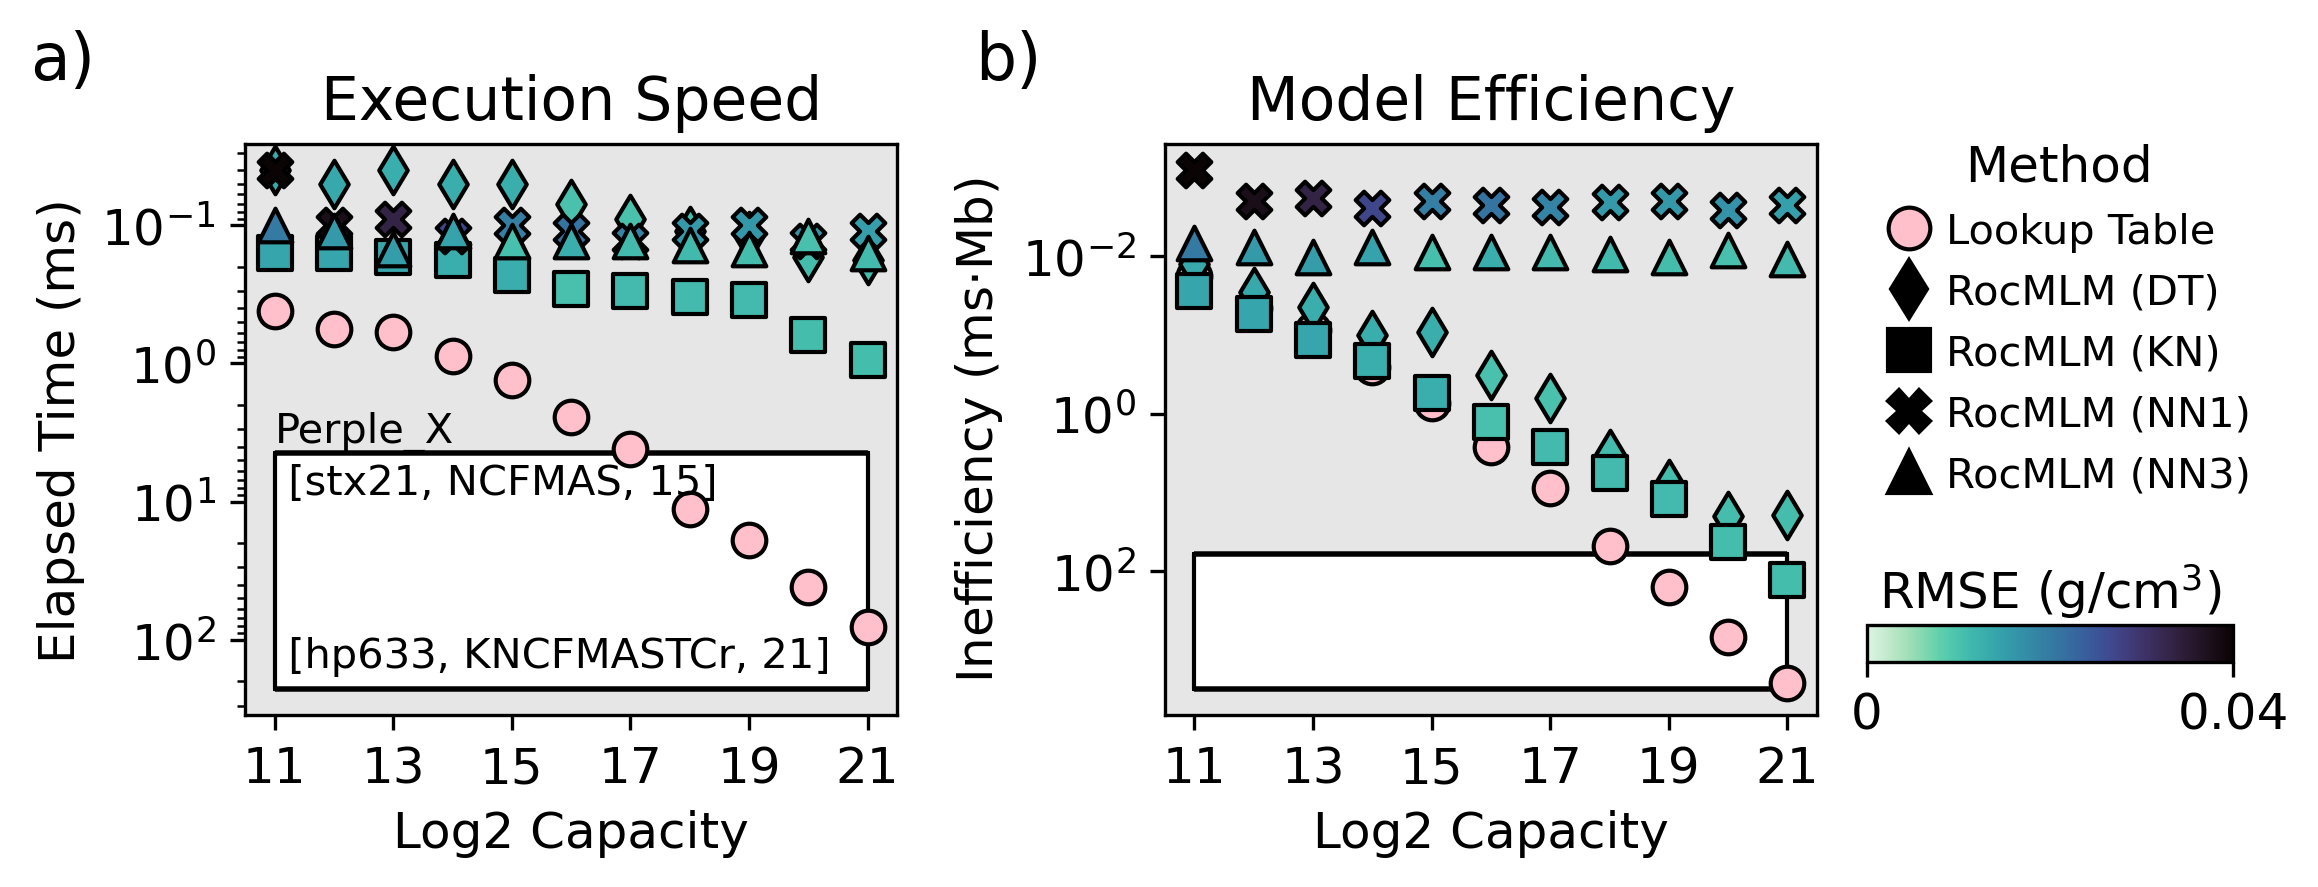
\includegraphics[width=1\linewidth,]{rocmlm-performance} 

}

\caption{Computational efficiency of various approaches in terms of execution speed (a) and model efficiency (b). ``Capacity'' (x-axis) is a proxy for the petrological ``knowledge'', or predictive capabilities, of Lookup Tables and RocMLMs. White regions indicate GFEM efficiencies for different Perple\_X configurations (thermodynamic dataset, chemical system, and number of solution phases are indicated in square brackets). stx21: \citet{stixrude2022}, hp633: \citet{holland2011} updated in \citet{holland2018}. Perple\_X was run without multilevel grid refinement. RMSE is measured between density predictions and the validation dataset.}\label{fig:rocmlm-performance}
\end{figure}

For Lookup Tables, execution speed and efficiency both scale roughly linearly with capacity on a logarithmic scale---indicating an inverse power-law relationship between Lookup Table capacity and performance (Figure \ref{fig:rocmlm-performance}). RocMLM performance, in contrast, scales differently depending on the performance metric and regression algorithm. For example, RocMLM execution speed remains roughly constant, or increasing slightly with capacity, and shows relatively small variance among all regression algorithms (0.14 ± 0.26 ms, 2\(\sigma\), Figure \ref{fig:rocmlm-performance}a). Yet RocMLM efficiency is markedly different for DT and KN algorithms compared to NN algorithms (Figure \ref{fig:rocmlm-performance}b). Despite the fast execution times of KN and DT algorithms (Figure \ref{fig:rocmlm-performance}a), their efficiency scales roughly linearly with capacity on a logarithmic scale---indicating an inverse power-law relationship between efficiency and capacity similar to Lookup Tables (Figure \ref{fig:rocmlm-performance}b). NN algorithms, on the other hand, show roughly constant efficiencies that indicate a high degree of information compression without sacrificing execution speed (Figure \ref{fig:rocmlm-performance}b). We note that training times for NN algorithms are many orders of magnitude larger than DT and KN algorithms (Supplementary Information). However, training times are neither limiting nor critical for geodynamic applications as training is independent from, and precedes numerical simulations.

Since accuracy is measured relative to the rock properties generated by GFEM programs, GFEM programs have perfect accuracy by definition. With respect to RocMLMs, validation accuracies (RMSE) are observed to be roughly constant for regression algorithms that apply binary decisions or local distance-based weights (DT and KN), while algorithms that apply global activation-based weights (NNs) show a positive correlation between accuracy and capacity (Figure \ref{fig:rocmlm-performance}). In addition to improving accuracy with increasing amounts of training examples, NN accuracy also increases with the number of hidden-layers (Figure \ref{fig:rocmlm-performance}) because deeper networks are more capable of fitting sharp gradients in the training data (see Supplementary Information for examples of NN1, NN2, and NN3 RocMLMs). We also tested the effects of NN width (changing the number of nodes within each hidden layer), but this had a negligible impact on NN performance and accuracy compared to increasing NN depth.

\section{Discussion}\label{discussion}

\subsection{RocMLM Performance Tradeoffs}\label{sec:rocmlms-tradeoffs}

RocMLM performance and accuracy are both critical for geodynamic applications and crucial for determining if RocMLMs are an improvement over methods commonly used for predicting rock properties in numerical geodynamic simulations. In terms of pure execution speed, our testing demonstrates that RocMLMs can make predictions between 10\(^1\)--10\(^3\) times faster than GFEM programs and Lookup Tables (Figure \ref{fig:rocmlm-performance}), depending on the GFEM program configuration. The difference in execution speed between Lookup Tables and RocMLMs is small for low-resolution models (Figure \ref{fig:rocmlm-performance}) that are limited to ≤ 16 mantle compositions and large PT intervals (≥ 1.7 GPa and 100 K PT step sizes). However, such low-resolution models are not an obvious improvement over simple polynomial approximations of a selective number of important phase transformations. At higher resolutions, RocMLMs can accurately resolve the physical properties of all thermodynamically-stable mineral assemblages in fine detail (at PT intervals of ≤ 0.2 GPa and 12 K) and for a wide variety of bulk mantle compositions (Figure \ref{fig:earthchem-mixing-array}). In addition to their broad predictive capabilities, high-resolution RocMLMs make predictions at speeds (approximately 0.1--1 ms, Figure \ref{fig:rocmlm-performance}) that allow computation of physical properties at the node-scale during geodynamic simulations. We therefore argue that high-resolution RocMLMs overcome all practical limitations for implementing thermodynamically self-consistent density evolution in numerical geodynamic models.

With respect to ranking the practicality of different RocMLM for geodynamic applications, execution speeds and accuracies alone suggest that high-resolution RocMLMs will perform with roughly equivalent outcomes regardless of the regression algorithm (Figure \ref{fig:rocmlm-performance}a). However, our testing reveals an obvious tradeoff between RocMLM performance and accuracy when accounting for compression ratio (i.e., the amount of ``learned'' information relative to the RocMLM file size). Figure \ref{fig:rocmlm-performance}b shows DT and KN algorithms becoming rapidly inefficient compared to NNs as the capacity of the training dataset increases. This is because NN algorithms require relatively little information to make predictions after training (weights and biases for each neuron) compared to DT (tree structure: nodes, splits, and predictions) and KN (entire training dataset with distance weights) algorithms. Moreover, accuracy tends to improve monotonically with dataset capacity for NN, but not for DT or KN. We therefore argue that deep NN RocMLMs are the most practical choice for geodynamic applications for three reasons: 1) modeling more rock types only requires adding more training data, 2) adding more training data improves prediction accuracy without diminishing performance, and 3) further improvements and adaptations to different geodynamic applications are possible by exploring different architectures than the simple NN models we have tested thus far.

The main limitations of NN RocMLMs are twofold: 1) training is computationally expensive compared to other regression algorithms (Supplementary Information) and 2) shallow NN architectures imply smoother gradients in rock properties than GFEM calculations. We do not consider these limitations critical because training time is independent from RocMLM performance and even if deeper NN architectures are needed to fit discontinuities in rock properties with high accuracy, the number of layers and neurons in each layer remains small (Table \ref{tab:rocmlm-config}). We note that our testing has been limited to the prediction of three properties that are mostly P-dependent and are relatively continuous despite a few large discontinuities. In principle, RocMLMs can be trained on any thermodynamic variable output by GFEM programs. However, we have not yet trained RocMLMs on more discrete, discontinuous, and/or highly T-dependent variables, such as modal proportions of minerals, volatile contents, or melt fraction, which will be treated in future developments of RocMLMs.

\subsection{Geophysical and Thermodynamic Estimates of Elastic Properties}\label{sec:rocmlm-elastic-properties}

The amount of overlap between RocMLM profiles and PREM (Figures \ref{fig:image12-PUM-DT}--\ref{fig:image12-PUM-DT}) suggests good agreement between thermodynamic and geophysical estimates of the elastic properties of mantle rocks within the limits of our training dataset and Perple\_X configuration (see Sections \ref{sec:training-data-design} and \ref{sec:generate-training-data}). Discrepancies between thermodynamic profiles and PREM can be explained by chemical heterogeneity and/or differences in mantle geotherms that modify phase relations \citep{goes2022, karki1999, karki2001, stixrude2012, waszek2021, xu2008}. Because the RocMLM training dataset spans a wide array of synthetic bulk mantle compositions, we can directly test the sensitivity of thermodynamic estimates to changes in bulk FeO--MgO contents (Figure \ref{fig:prem-comps}).

As Fertility Index (\(\xi\)) increases by refertilization and/or lack of melt extraction and the bulk mantle composition becomes more Fe-rich (and more dense), Vp and Vs respond (both positively and negatively) according to the equations of state described in \citet{stixrude2005}. RocMLM training data show that density is the least sensitive parameter to \(\xi\) overall with only modest variations across a broad range of mantle rocks from fertile to highly depleted (\(\xi\) = 0.76, Figure \ref{fig:prem-comps}a). The largest density variations occur at pressures below the olivine → wadsleyite transition (\textless{} 410 km), yet are still small enough (approximately 3--5 \%) to imply that spontaneous mantle convection requires strong thermal gradients and/or hydration by metamorphic fluids in addition to melt extraction.

In contrast to density, Vp and Vs are more sensitive to \(\xi\) overall, especially at pressures above the olivine → wadsleyite transition (\textgreater{} 410 km). RocMLM training data suggests that an ``optimal'' Vp/Vs profile requires a more depleted mantle between 410--670 km and a more fertile mantle at \textless{} 410 km (Figure \ref{fig:prem-comps}b,c). Forming this compositional layering pattern is counterintuitive, however, as partial melting is expected to be more pervasive at lower pressures. Moreover, density profiles are incongruent with this pattern, suggesting instead that a depleted mantle at \textless{} 410 km and more fertile mantle at \textgreater{} 410 km are required for an optimal fit with PREM and STW105 (Figure \ref{fig:prem-comps}a).



\begin{figure}[htbp]

{\centering 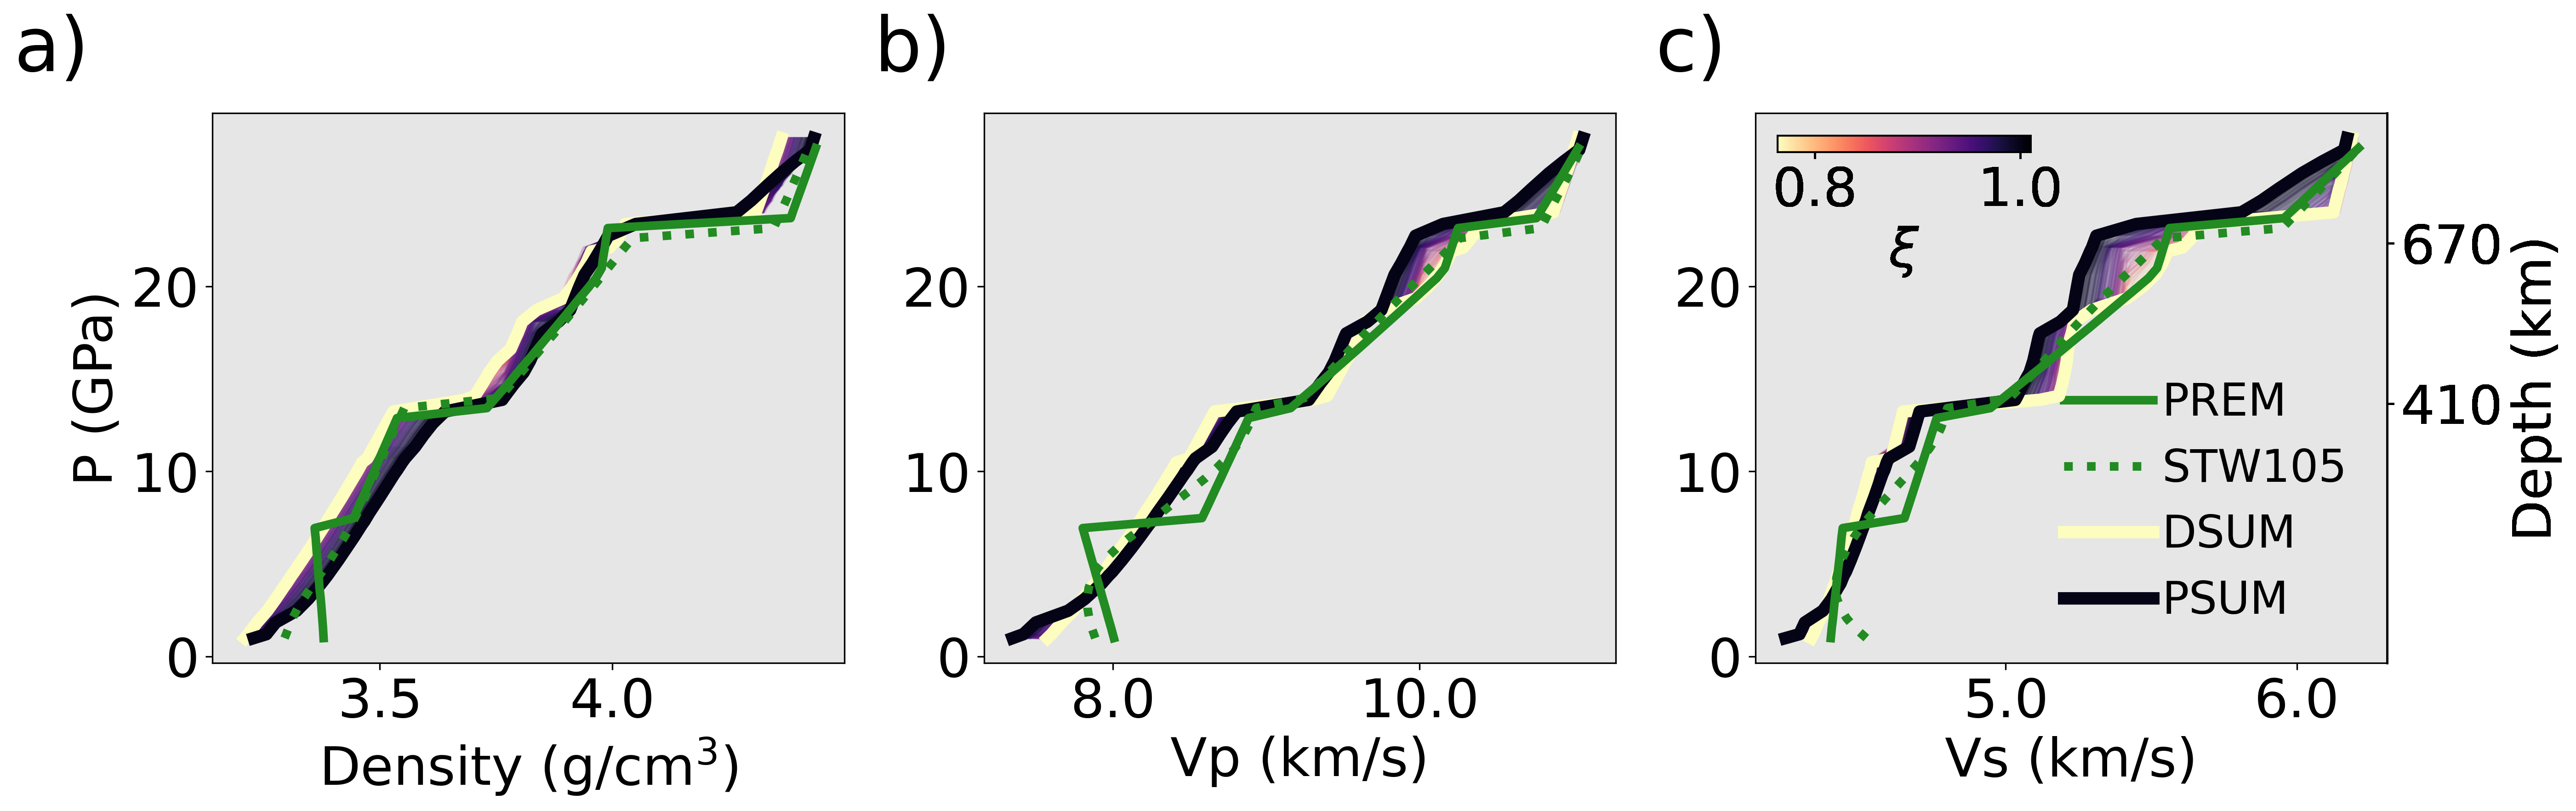
\includegraphics[width=1\linewidth,]{prem-comps} 

}

\caption{Depth profiles of RocMLM training data along a 1573 K mantle adiabat showing the sensitivities of thermodynamic estimates of density (a), Vp (b), and Vs (c) to changes in bulk mantle composition (as represented by the Fertility Index, \(\xi\)). Geophysical profiles PREM and STW105 (green lines) and the profiles of synthetic mantle end-member compositions PSUM and DSUM (thick colored lines) are shown for reference. Thin colored lines show profiles for the entire range of RocMLM training data.}\label{fig:prem-comps}
\end{figure}

\section{Conclusions}\label{conclusions}

The dynamics of Earth's upper mantle is largely driven by density contrasts stemming from changes in PT conditions, which lead to phase transformations in mantle rocks. These phase transformations also modify the elastic properties of mantle rocks. Therefore phase changes must be considered when inverting present-day mantle structure from seismic data. Likewise, numerical geodynamic simulations of mantle convection must account for thermodynamics, but are typically implemented with simple PT-dependent parameterizations of rock properties and phase boundaries that do not explicitly account for changes in Gibbs Free Energy resulting from changes in PT and in bulk composition. Here, we introduce RocMLMs as an alternative to GFEM programs and we evaluate RocMLM performance and accuracy. We also show how the RocMLM predictions compare to PREM and STW105. Our main findings are as follows:

\begin{enumerate}
\def\labelenumi{\arabic{enumi}.}
\tightlist
\item
  RocMLMs predict density and elastic properties with high accuracy and are up to 101--103 faster than commonly used methods. This improvement in prediction speed makes thermodynamically self-consistent mantle convection within high-resolution numerical geodynamic models practical for the first time.
\item
  RocMLMs trained with moderately deep (3 hidden layers) NNs are more robust and efficient compared to RocMLMs trained with other regression algorithms, and are therefore the most practical models for coupling with numerical geodynamic codes.
\item
  RocMLM training data are sensitive to bulk mantle composition and geothermal gradients, yet show good agreement with PREM and STW105 for an average mantle geotherm.
\end{enumerate}

Based on our results, we argue that moderately deep NN RocMLMs can be exceptional emulators of GFEM programs in geodynamic simulations that require computationally efficient predictions of rock properties. We have demonstrated that RocMLMs perform remarkably well for dry mantle rocks with compositions ranging from very fertile lherzolites to strongly depleted harzburgites and PT conditions ranging from 1--28 GPa and 773--2273 K.

Moreover, the RocMLM approach can be used with any GFEM program and thermodynamic dataset. Any improvement to the underlying thermodynamic data should further increase the accuracy of RocMLM predictions. Testing RocMLMs predictions on other thermodynamic variables of interest, including modal proportions of minerals, volatile contents, and melt fractions will be the focus of future studies. Likewise, in future works, we will extend the training data to include hydrous systems and additional end-member mantle compositions (e.g., pyroxenites and dunites).

\section{Acknowledgements}\label{acknowledgements}

This work was supported by the Tremplin-ERC grant LEARNING awarded to Nestor Cerpa by the I-SITE excellence program at the Université de Montpellier. We thank Maurine Montagnat, Fernando Carazo, Nicolas Berlie, and many researchers and students at Géosciences Montpellier for their thoughtful feedback during the development of this work. We gratefully acknowledge additional support from the European Research Council (ERC) under the European Union Horizon 2020 Research and Innovation program grant agreement No.~882450 (ERC RhEoVOLUTION) awarded to Andréa Tommasi.

\section{Open Research}\label{open-research}

All data, code, and relevant information for reproducing this work can be found at \url{https://github.com/buchanankerswell/kerswell_et_al_rocmlm}, and at \url{https://doi.org/10.17605/OSF.IO/K23TB}, the official Open Science Framework data repository \citep{kerswell2024}. All code is MIT Licensed and free for use and distribution (see license details). Reference models PREM and STW105 are freely available from the Incorporated Research Institutions for Seismology Earth Model Collaboration \citep[IRIS EMC, doi: 10.17611/DP/EMC.1,][]{trabant2012}. All computations were made using CPUs of a Macbook Pro (2022; M2 chip) with macOS 13.4 and using Python 3.11.4.

\section{References}\label{references}

\cleardoublepage

\bibliography{main.bib}


\end{document}
